\documentclass{report}

\usepackage[utf8]{inputenc}
\usepackage[T1]{fontenc}
\usepackage[francais]{babel}
\usepackage{graphicx}
\usepackage{circuitikz}
\usepackage[squaren, Gray]{SIunits}
\usepackage{sistyle}
\usepackage[autolanguage]{numprint}
\usepackage{pgfplots}
\pgfplotsset{compat=1.9}
\usepackage{amsmath,amssymb,array}
\usepackage[top=2.5cm,bottom=2.5cm,right=2.5cm,left=2.5cm]{geometry}
\DeclareMathOperator{\dist}{d}
\usepackage{multibib}
\newenvironment{abstract-fr}
{
	\begin{center}
		\textbf{Résumé} \\[0.5cm]
	\end{center}
}
{}

\newenvironment{abstract-en}
{
	\begin{center}
		\textbf{Summary} \\[0.5cm]
	\end{center}
}
{}
% New command pour la modélisation mécanique, tri à effectuer
\newcommand\fv[1]{{\bf #1}} % free vector
\newcommand\fvd[1]{\dot{\bf #1}} % free vector derivated
\newcommand\fvdd[1]{\ddot{\bf #1}} % free vector derivated
\newcommand\fvr[1]{\mathring{\bf #1}} % free vector relatively derivated
\newcommand\fvrr[1]{\overset{\circ\circ}{\bf #1}} % free vector relatively derivated
\newcommand\uv[1]{{\bf\hat{ #1}}} % unit vector
\newcommand\ui{{\bf\hat{I}}} % unit vector I
\newcommand\uj{{\bf\hat{J}}} % unit vector J
\newcommand\uk{{\bf\hat{K}}} % unit vector K
\newcommand\wrt[2]{\ensuremath{\tensor*[_{ #1}]{ #2}{}}} % With Respect To
\newcommand\wtr[3]{\ensuremath{\tensor*[_{ #1}]{ #2}{^{ #3}}}} % With Two Respect
\newcommand\omegaf{{\bm \omega}}
\newcommand\omegafr{\mathring{\bm \omega}}
\newcommand\omegafd{\dot{\bm \omega}}
\newcommand\omegaft{\tilde{\bm \omega}}
\newcommand\omegaftr{\mathring{\tilde{\bm \omega}}}
\newcommand\omegat{\tilde{\omega}}
\newcommand\omegatd{\tilde{\dot{\omega}}}
\newcommand\ine{{\bf I}}
\newcommand\st{{\bf L}}
\newcommand\pst{{\bf M}}
\newcommand\lm{{\bf N}}
\newcommand\am{{\bf H}}
\newcommand\amd{\dot{\am}}
\newcommand\fo{{\bf F}}
\newcommand\po{\mathcal{P}}
\newcommand\xg{\ensuremath{\fv{R}}}
\newcommand\xgd{\ensuremath{\fvd{R}}}
\newcommand\xgdd{\ensuremath{\fvdd{R}}}
\newcommand\dvec[1]{\dot{\vec{ #1}}}
\newcommand\ddvec[1]{\ddot{\vec{ #1}}}
\newcommand\qp{\dot{q}}
\newcommand\dqp{\Delta \dot{q}}
\usepackage{url} 
\usepackage{hyperref}
\hypersetup{
    colorlinks,
    citecolor=black,
    filecolor=black,
    linkcolor=black,
    urlcolor=black
}

\begin{document}

% Page de garde
\begin{titlepage}
\begin{center}


\includegraphics[width=0.15\textwidth]{logo.jpg}~\\[1cm]

\textsc{\LARGE Ecole Polytechnique de Louvain-La-Neuve}\\[1.5cm]

\textsc{\Large FSAB1502 - Projet 2}\\[0.5cm]

% Title
\HRule \\[0.4cm]
{\huge \bfseries Concevoir, réaliser et qualifier un système de haut-parleur\\[0.5cm]}

\HRule \\[1.5cm]

\begin{minipage}{1.0\textwidth}
\begin{flushleft} \large
\emph{Auteurs : } Groupe \numprint{115.3}\\[0.2cm]

\begin{tabular}{lr}
Thibaut \textsc{Cabo} & (\numprint{4353-1300}) \\
Lise \textsc{Céresiat} & (\numprint{1965-1200}) \\
Robin \textsc{Crits} & (\numprint{3236-1300}) \\
Virgile \textsc{Goyens} & (\numprint{8339-1300}) \\
Antoine \textsc{Paris} & (\numprint{3158-1300}) \\
Marie-Charlotte \textsc{Sparenberg} & (\numprint{5408-1300})
\end{tabular}

\end{flushleft}
\end{minipage}

\HRule \\[1.0cm]

\begin{minipage}{1.0\textwidth}
\begin{flushleft} \large
\emph{Tuteur :} \\[0.2cm]
\begin{tabular}{l}
Pr.~Piotr \textsc{Sobieski}
\end{tabular}
\end{flushleft}
\end{minipage}

\vfill

{\large \today}

\end{center}
\end{titlepage}

% Abstract
\documentclass{article}

\usepackage[utf8]{inputenc}
\usepackage[T1]{fontenc}      
\usepackage[francais]{babel}
\usepackage{graphicx}
\usepackage{circuitikz}
\usepackage[squaren, Gray]{SIunits}
\usepackage{sistyle}
\usepackage[autolanguage]{numprint}
\usepackage{pgfplots}
\pgfplotsset{compat=1.9}
\usepackage{amsmath,amssymb,array}
\usepackage[top=2.5cm,bottom=2.5cm,right=2.5cm,left=2.5cm]{geometry}
\usepackage{url} 
\usepackage{tabularx}
\DeclareMathOperator{\dist}{d}
\newenvironment{abstract-fr}
{
	\begin{center}
		\textbf{Résumé} \\[0.5cm]
	\end{center}
}
{}

\newenvironment{abstract-en}
{
	\begin{center}
		\textbf{Summary} \\[0.5cm]
	\end{center}
}
{}
% New command pour la modélisation mécanique, tri à effectuer
\newcommand\fv[1]{{\bf #1}} % free vector
\newcommand\fvd[1]{\dot{\bf #1}} % free vector derivated
\newcommand\fvdd[1]{\ddot{\bf #1}} % free vector derivated
\newcommand\fvr[1]{\mathring{\bf #1}} % free vector relatively derivated
\newcommand\fvrr[1]{\overset{\circ\circ}{\bf #1}} % free vector relatively derivated
\newcommand\uv[1]{{\bf\hat{ #1}}} % unit vector
\newcommand\ui{{\bf\hat{I}}} % unit vector I
\newcommand\uj{{\bf\hat{J}}} % unit vector J
\newcommand\uk{{\bf\hat{K}}} % unit vector K
\newcommand\wrt[2]{\ensuremath{\tensor*[_{ #1}]{ #2}{}}} % With Respect To
\newcommand\wtr[3]{\ensuremath{\tensor*[_{ #1}]{ #2}{^{ #3}}}} % With Two Respect
\newcommand\omegaf{{\bm \omega}}
\newcommand\omegafr{\mathring{\bm \omega}}
\newcommand\omegafd{\dot{\bm \omega}}
\newcommand\omegaft{\tilde{\bm \omega}}
\newcommand\omegaftr{\mathring{\tilde{\bm \omega}}}
\newcommand\omegat{\tilde{\omega}}
\newcommand\omegatd{\tilde{\dot{\omega}}}
\newcommand\ine{{\bf I}}
\newcommand\st{{\bf L}}
\newcommand\pst{{\bf M}}
\newcommand\lm{{\bf N}}
\newcommand\am{{\bf H}}
\newcommand\amd{\dot{\am}}
\newcommand\fo{{\bf F}}
\newcommand\po{\mathcal{P}}
\newcommand\xg{\ensuremath{\fv{R}}}
\newcommand\xgd{\ensuremath{\fvd{R}}}
\newcommand\xgdd{\ensuremath{\fvdd{R}}}
\newcommand\dvec[1]{\dot{\vec{ #1}}}
\newcommand\ddvec[1]{\ddot{\vec{ #1}}}
\newcommand\qp{\dot{q}}
\newcommand\dqp{\Delta \dot{q}}
\usepackage{url} 
\usepackage{hyperref}
\hypersetup{
    colorlinks,
    citecolor=black,
    filecolor=black,
    linkcolor=black,
    urlcolor=black
}

\begin{document}

\begin{abstract-fr}
% Contexe et tâche
Dans le cadre du cours \textit{Projet 2}, il nous a été demandé
de concevoir un haut-parleur que l'on puisse connecter à un smartphone
par le biais d'une prise Jack.
% Besoin
Pour arrivers à nos fins, il a fallu passer par diverses étapes
de modélisations mathématiques et physiques de composants du haut-
parleur. Les situations réelles étant en général trop compliquées à étudier
dans leur globalité (en tout cas à notre stade), ces modèlisations se basent sur des hypothèses simplificatrices. Malgré que ces hypothèses soient parfois assez fortes, 
elles permettent d'arriver à un modèle relativement cohérent avec les expériences et
mesures effectuées en laboratoire.
% Objet
Ce document décrit en détail chacune des étapes de modélisation effectuée durant
ce projet. Il présente aussi une synthèse des différentes recherches documentaires.
% Résultats, conclusions et perspectives
Bien que notre haut-parleur ne fonctionne pas aussi bien que nous l'aurions
espéré, nous avons énomément appris de ce projet.
% To do : il manque une petite phrase mais je ne trouve pas.

\end{abstract-fr}

% Just here to fix rapport_prejury.tex
\end{document}

\documentclass{article}

\usepackage[utf8]{inputenc}
\usepackage[T1]{fontenc}      
\usepackage[francais]{babel}
\usepackage{graphicx}
\usepackage{circuitikz}
\usepackage[squaren, Gray]{SIunits}
\usepackage{sistyle}
\usepackage[autolanguage]{numprint}
\usepackage{pgfplots}
\pgfplotsset{compat=1.9}
\usepackage{amsmath,amssymb,array}
\usepackage[top=2.5cm,bottom=2.5cm,right=2.5cm,left=2.5cm]{geometry}
\usepackage{url} 
\usepackage{tabularx}
\DeclareMathOperator{\dist}{d}
\newenvironment{abstract-fr}
{
	\begin{center}
		\textbf{Résumé} \\[0.5cm]
	\end{center}
}
{}

\newenvironment{abstract-en}
{
	\begin{center}
		\textbf{Summary} \\[0.5cm]
	\end{center}
}
{}
% New command pour la modélisation mécanique, tri à effectuer
\newcommand\fv[1]{{\bf #1}} % free vector
\newcommand\fvd[1]{\dot{\bf #1}} % free vector derivated
\newcommand\fvdd[1]{\ddot{\bf #1}} % free vector derivated
\newcommand\fvr[1]{\mathring{\bf #1}} % free vector relatively derivated
\newcommand\fvrr[1]{\overset{\circ\circ}{\bf #1}} % free vector relatively derivated
\newcommand\uv[1]{{\bf\hat{ #1}}} % unit vector
\newcommand\ui{{\bf\hat{I}}} % unit vector I
\newcommand\uj{{\bf\hat{J}}} % unit vector J
\newcommand\uk{{\bf\hat{K}}} % unit vector K
\newcommand\wrt[2]{\ensuremath{\tensor*[_{ #1}]{ #2}{}}} % With Respect To
\newcommand\wtr[3]{\ensuremath{\tensor*[_{ #1}]{ #2}{^{ #3}}}} % With Two Respect
\newcommand\omegaf{{\bm \omega}}
\newcommand\omegafr{\mathring{\bm \omega}}
\newcommand\omegafd{\dot{\bm \omega}}
\newcommand\omegaft{\tilde{\bm \omega}}
\newcommand\omegaftr{\mathring{\tilde{\bm \omega}}}
\newcommand\omegat{\tilde{\omega}}
\newcommand\omegatd{\tilde{\dot{\omega}}}
\newcommand\ine{{\bf I}}
\newcommand\st{{\bf L}}
\newcommand\pst{{\bf M}}
\newcommand\lm{{\bf N}}
\newcommand\am{{\bf H}}
\newcommand\amd{\dot{\am}}
\newcommand\fo{{\bf F}}
\newcommand\po{\mathcal{P}}
\newcommand\xg{\ensuremath{\fv{R}}}
\newcommand\xgd{\ensuremath{\fvd{R}}}
\newcommand\xgdd{\ensuremath{\fvdd{R}}}
\newcommand\dvec[1]{\dot{\vec{ #1}}}
\newcommand\ddvec[1]{\ddot{\vec{ #1}}}
\newcommand\qp{\dot{q}}
\newcommand\dqp{\Delta \dot{q}}
\usepackage{url} 
\usepackage{hyperref}
\hypersetup{
    colorlinks,
    citecolor=black,
    filecolor=black,
    linkcolor=black,
    urlcolor=black
}

\begin{document}

\begin{abstract-en}


In this course, \textit{Projet 2}, it has been asked to make a loud-speaker that can be connected to a smartphone with a Jack-plug.

To achieve this task, we had to work out to find a way to go through it.  We had to find simpler mathematical and physical models.  
The real problem was too tricky for us so we had to make some simpler assumptions.  However, we couldn't make random assumption because the theorie has to fit with the test we did in the lab.

In this document, you'll find the necessary calculations and ideas to make such a tool.

Even if our loud-speaker doesn't work as well as we wanted, we learned a lot from this challenge. 

Our state of mind is pretty hard to describe: we are disappointed with the actual loud-speaker but quite proud of us for the rest.


\end{abstract-en}

% Just here to fix rapport_prejury.tex
\end{document}


\clearpage
\tableofcontents
\clearpage

\chapter{Introduction}

\documentclass{article}

\usepackage[utf8]{inputenc}
\usepackage[T1]{fontenc}      
\usepackage[francais]{babel}
\usepackage{graphicx}
\usepackage{circuitikz}
\usepackage[squaren, Gray]{SIunits}
\usepackage{sistyle}
\usepackage[autolanguage]{numprint}
\usepackage{pgfplots}
\pgfplotsset{compat=1.9}
\usepackage{amsmath,amssymb,array}
\usepackage[top=2.5cm,bottom=2.5cm,right=2.5cm,left=2.5cm]{geometry}
\usepackage{url} 
\usepackage{tabularx}
\DeclareMathOperator{\dist}{d}
\newenvironment{abstract-fr}
{
	\begin{center}
		\textbf{Résumé} \\[0.5cm]
	\end{center}
}
{}

\newenvironment{abstract-en}
{
	\begin{center}
		\textbf{Summary} \\[0.5cm]
	\end{center}
}
{}
% New command pour la modélisation mécanique, tri à effectuer
\newcommand\fv[1]{{\bf #1}} % free vector
\newcommand\fvd[1]{\dot{\bf #1}} % free vector derivated
\newcommand\fvdd[1]{\ddot{\bf #1}} % free vector derivated
\newcommand\fvr[1]{\mathring{\bf #1}} % free vector relatively derivated
\newcommand\fvrr[1]{\overset{\circ\circ}{\bf #1}} % free vector relatively derivated
\newcommand\uv[1]{{\bf\hat{ #1}}} % unit vector
\newcommand\ui{{\bf\hat{I}}} % unit vector I
\newcommand\uj{{\bf\hat{J}}} % unit vector J
\newcommand\uk{{\bf\hat{K}}} % unit vector K
\newcommand\wrt[2]{\ensuremath{\tensor*[_{ #1}]{ #2}{}}} % With Respect To
\newcommand\wtr[3]{\ensuremath{\tensor*[_{ #1}]{ #2}{^{ #3}}}} % With Two Respect
\newcommand\omegaf{{\bm \omega}}
\newcommand\omegafr{\mathring{\bm \omega}}
\newcommand\omegafd{\dot{\bm \omega}}
\newcommand\omegaft{\tilde{\bm \omega}}
\newcommand\omegaftr{\mathring{\tilde{\bm \omega}}}
\newcommand\omegat{\tilde{\omega}}
\newcommand\omegatd{\tilde{\dot{\omega}}}
\newcommand\ine{{\bf I}}
\newcommand\st{{\bf L}}
\newcommand\pst{{\bf M}}
\newcommand\lm{{\bf N}}
\newcommand\am{{\bf H}}
\newcommand\amd{\dot{\am}}
\newcommand\fo{{\bf F}}
\newcommand\po{\mathcal{P}}
\newcommand\xg{\ensuremath{\fv{R}}}
\newcommand\xgd{\ensuremath{\fvd{R}}}
\newcommand\xgdd{\ensuremath{\fvdd{R}}}
\newcommand\dvec[1]{\dot{\vec{ #1}}}
\newcommand\ddvec[1]{\ddot{\vec{ #1}}}
\newcommand\qp{\dot{q}}
\newcommand\dqp{\Delta \dot{q}}
\usepackage{url} 
\usepackage{hyperref}
\hypersetup{
    colorlinks,
    citecolor=black,
    filecolor=black,
    linkcolor=black,
    urlcolor=black
}

\begin{document}

% L'objectif du projet + les spécifications attendues + cahier des charges (ref)
Dans le cadre du cours \textit{Projet 2} du deuxième quadrimestre, notre groupe a été amené à 
concevoir un haut-parleur connectable, via une prise Jack \unit{3.5}{\milli\meter}, à un 
GSM ou un MP3 (les contraintes et spécifications sont détaillées dans l'annexe ''Cahier des charges''). 
En plus de cela, notre haut-parleur doit permette un règlage du volume, des graves
et des aigus. Un autre objectif du projet est d'apprendre un travailler et à s'organiser \textit{en groupe}, 
comme le font tous les jours les ingénieurs.

% L'organisation du rapport
Ce rapport s'articule principalement en deux grands chapitres. Le premier
rassemble les différentes étapes de modélisations mathématiques
et physiques de composants du haut-parleur. Dans ce chapitre, nous 
commencerons par une vue générale du haut-parleur qui nous
permettra d'introduire les concepts physiques clés. Nous continuerons
ensuite par la modélisation des filtres passe-bas, passe-haut et passe bande.
Après cela, nous nous attarderons  sur le dimensionnement de l'électroaimant et
de la bobine mobile pour enfin terminer par la modélisation mécanique de la bobine
mobile.

Le deuxième chapitre contient quant à lui la synthèse des recherches documentaires
effectuées. Ces recherches portent sur deux sujets liés à notre haut-parleur. Le premier
concerne plutôt l'acoustique, il s'agit de la 
distorsion harmonique. Le deuxième quant à lui concerne un concept lié au circuit électrique qui
compose notre haut-parleur, il s'agit du principe de la contre-réaction.

% Description générale du système
Penchons-nous sans plus tarder sur une description générale du système. Notre haut-parleur
peut-être représenté schématiquement comme sur la Figure \ref{block-diagram-hp}.

% Schéma montrant le bonne compréhension du système
\begin{figure}[!htb]
	\centering
	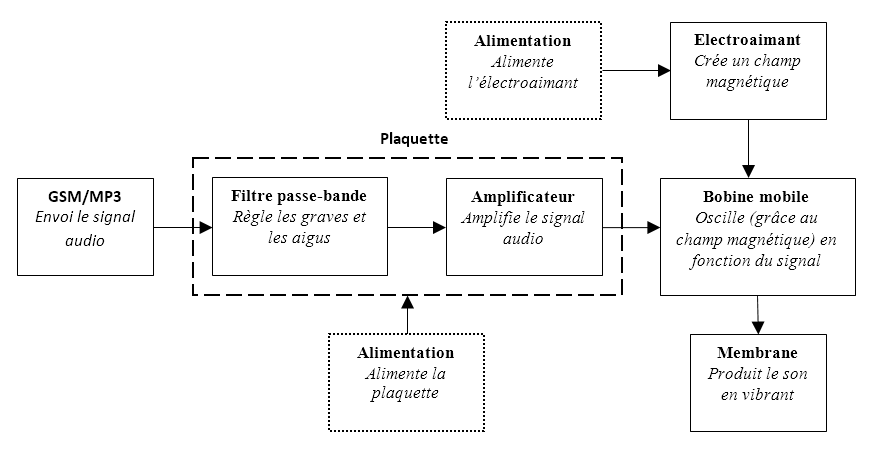
\includegraphics[scale=0.68]{schema_fonctionnel.png}
	\caption{Schéma fonctionnel du haut-parleur.}
	\label{block-diagram-hp}
\end{figure}

Le GSM ou le MP3 va dans un premier temps envoyé un signal audio via le cable Jack au circuit
imprimé, par la suite nous qualifierons ce signal de \textit{brute}. Le circuit imprimé permet
quant à lui de modifier ce signal brute de plusieurs façon : 

\begin{itemize}
	\item En règlant le volume, c'est à dire en modifiant l'amplitude du signal audio ;
	\item En règlant les graves et les aigus, c'est à dire en atténuant les basses ou les hautes
	fréquences. Il s'agit du rôle des filtres passe-bas et passe-haut qui combiné forme un filtre 
	passe-bande ;
	\item En amplifiant le signal : c'est le rôle de l'amplifcateur audio du circuit.
\end{itemize}

A la sortie du circuit imprimé, le signal est alors \textit{filtré} et \textit{amplifié}.
Ce signal traité ira ensuite alimenter en courant la bobine mobile. Cette 
dernière intercepte un champ magnétique constant, noté $B$, produit par l'électroaimant.
L'électroaimant est constitué de fines lamelles de matériau magnétique en forme de ''E'' 
empilé les unes sur les autres. La perméabilité magnétique élevé de ce matériau
($\mu_r \approx \ 1600$) permet de créer un champ magnétique plus fort. Autour de la branche
centrale du ''E'' est enroulée du fil de cuivre, formant ainsi une bobine.
La bobine mobile subit donc une force de \textsc{Laplace} dont l'expression est :

$$\vec{F} = i(t)\vec{L}\times{\vec{B}}$$ 

Où $L$ est la longueur du fil et$i(t)$ le courant le traversant. Cette force est proportionnelle
au courant traversant
la bobine mobile. La membrane se déplacera donc de manière cohérente avec le signal audio
et reproduira le son voulu. Enfin, la membrane pourra revenir à son position d'équilibre
grâce à des attaches qui, à la manière de ressorts, produisent une force de rappel.

% Just here to fix rapport_prejury.tex
\end{document}

\chapter{Fonctionnement du haut-parleur}

\documentclass{article}

\usepackage[utf8]{inputenc}
\usepackage[T1]{fontenc}      
\usepackage[francais]{babel}
\usepackage{graphicx}
\usepackage{circuitikz}
\usepackage[squaren, Gray]{SIunits}
\usepackage{sistyle}
\usepackage[autolanguage]{numprint}
\usepackage{pgfplots}
\pgfplotsset{compat=1.9}
\usepackage{amsmath,amssymb,array}
\usepackage[top=2.5cm,bottom=2.5cm,right=2.5cm,left=2.5cm]{geometry}
\usepackage{url} 
\usepackage{tabularx}
\DeclareMathOperator{\dist}{d}
\newenvironment{abstract-fr}
{
	\begin{center}
		\textbf{Résumé} \\[0.5cm]
	\end{center}
}
{}

\newenvironment{abstract-en}
{
	\begin{center}
		\textbf{Summary} \\[0.5cm]
	\end{center}
}
{}
% New command pour la modélisation mécanique, tri à effectuer
\newcommand\fv[1]{{\bf #1}} % free vector
\newcommand\fvd[1]{\dot{\bf #1}} % free vector derivated
\newcommand\fvdd[1]{\ddot{\bf #1}} % free vector derivated
\newcommand\fvr[1]{\mathring{\bf #1}} % free vector relatively derivated
\newcommand\fvrr[1]{\overset{\circ\circ}{\bf #1}} % free vector relatively derivated
\newcommand\uv[1]{{\bf\hat{ #1}}} % unit vector
\newcommand\ui{{\bf\hat{I}}} % unit vector I
\newcommand\uj{{\bf\hat{J}}} % unit vector J
\newcommand\uk{{\bf\hat{K}}} % unit vector K
\newcommand\wrt[2]{\ensuremath{\tensor*[_{ #1}]{ #2}{}}} % With Respect To
\newcommand\wtr[3]{\ensuremath{\tensor*[_{ #1}]{ #2}{^{ #3}}}} % With Two Respect
\newcommand\omegaf{{\bm \omega}}
\newcommand\omegafr{\mathring{\bm \omega}}
\newcommand\omegafd{\dot{\bm \omega}}
\newcommand\omegaft{\tilde{\bm \omega}}
\newcommand\omegaftr{\mathring{\tilde{\bm \omega}}}
\newcommand\omegat{\tilde{\omega}}
\newcommand\omegatd{\tilde{\dot{\omega}}}
\newcommand\ine{{\bf I}}
\newcommand\st{{\bf L}}
\newcommand\pst{{\bf M}}
\newcommand\lm{{\bf N}}
\newcommand\am{{\bf H}}
\newcommand\amd{\dot{\am}}
\newcommand\fo{{\bf F}}
\newcommand\po{\mathcal{P}}
\newcommand\xg{\ensuremath{\fv{R}}}
\newcommand\xgd{\ensuremath{\fvd{R}}}
\newcommand\xgdd{\ensuremath{\fvdd{R}}}
\newcommand\dvec[1]{\dot{\vec{ #1}}}
\newcommand\ddvec[1]{\ddot{\vec{ #1}}}
\newcommand\qp{\dot{q}}
\newcommand\dqp{\Delta \dot{q}}
\usepackage{url} 
\usepackage{hyperref}
\hypersetup{
    colorlinks,
    citecolor=black,
    filecolor=black,
    linkcolor=black,
    urlcolor=black
}

\begin{document}

\section{Fonctionnement général}
% Description générale du système + concepts physiques clés
Notre haut-parleur peut être représenté schématiquement comme sur la Figure \ref{block-diagram-hp}.

% Schéma montrant le bonne compréhension du système
\begin{figure}[!htb]
	\centering
	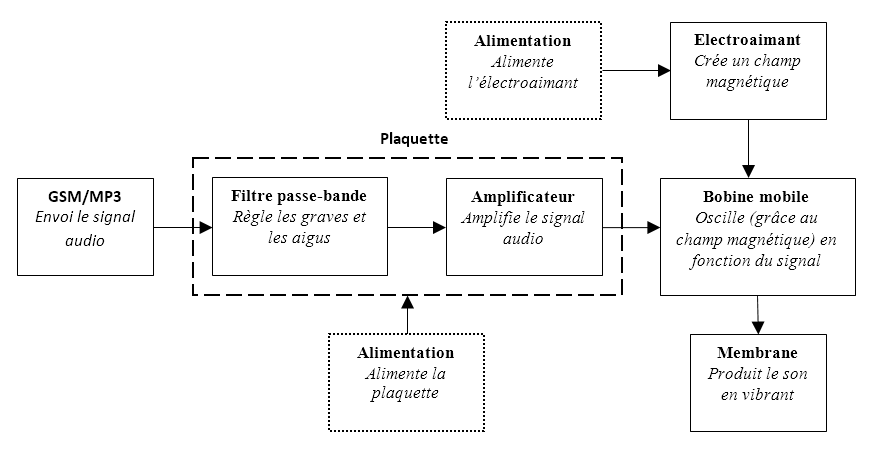
\includegraphics[scale=0.9]{schema_fonctionnel.png}
	\caption{Schéma fonctionnel du haut-parleur.}
	\label{block-diagram-hp}
\end{figure}

Le GSM ou le MP3 va dans un premier temps envoyer un signal audio via le câble Jack au circuit
imprimé; par la suite nous qualifierons ce signal de \textit{brut}. Le circuit imprimé permet
quant à lui de modifier ce signal brut de plusieurs façons : 

\begin{itemize}
	\item En réglant le volume, c'est-à-dire en modifiant l'amplitude du signal audio ;
	\item En réglant les graves et les aigus, c'est-à-dire en atténuant les basses fréquences
	(rôle du filtre passe-haut, circuit CR) ou les hautes
	fréquences (rôle du filtre passe-bas, circuit RC). Il s'agit du rôle des filtres passe-bas 
	et passe-haut qui,  combinés, forment un filtre passe-bande ;
	\item En amplifiant le signal : c'est le rôle de l'amplificateur audio du circuit.
\end{itemize}

À la sortie du circuit imprimé, le signal est alors \textit{filtré} et \textit{amplifié}.
Ce signal traité ira ensuite alimenter en courant la bobine mobile. Cette 
dernière intercepte un champ magnétique constant, noté $B$, produit par l'électroaimant.
L'électroaimant est constitué de fines lamelles de matériau magnétique en forme de ''E'' 
empilées les unes sur les autres. La perméabilité magnétique élevée de ce matériau
($\mu_r \approx \ 1600$) permet de créer un champ magnétique plus fort. Autour de la branche
centrale du ''E'' est enroulé du fil de cuivre, formant ainsi une bobine.
% Premier concept physique, loi d'Ampère
Le champ magnétique $B$ produit par l'électroaimant dans l'entrefer peut être calculé par la 
loi d'\textsc{Ampère} :

$$\vec{B} = \mu_0\mu_r\frac{NI}{e}\vec{u}$$

Où $N$ est le nombre de spires, $I$ le courant traversant la bobine et $e$ la largeur de 
l'entefer.

% Deuxième concept physique, force de Laplace
La bobine mobile subit donc une force de \textsc{Laplace} dont l'expression est :

$$\vec{F} = i(t)\vec{L}\times{\vec{B}}$$ 

Où $L$ est la longueur du fil et $i(t)$ le courant le traversant. Cette force est proportionnelle
au courant traversant
la bobine mobile. La membrane se déplacera donc de manière cohérente avec le signal audio
et reproduira le son voulu. Enfin, la membrane pourra revenir à sa position d'équilibre
grâce à des attaches qui, à la manière de ressorts, produisent une force de rappel dans la
direction opposée au mouvement de la bobine mobile :

$$\vec{F} = -k \vec{x}$$ % Troisième concept physique, loi d'Hook

Où $k$ est la constante de raideur des attaches et $x$ est le déplacement de la bobine mobile
par rapport à sa position d'origine (et donc la compression des attaches).

\paragraph{Remarque}
Une description plus détaillée de chaque composant du circuit électrique est présentée
dans l'annexe ''Analyse séquentielle du circuit''.

% Just here to fix rapport_prejury.tex
\end{document}

\clearpage

\documentclass{article}

\usepackage[utf8]{inputenc}
\usepackage[T1]{fontenc}      
\usepackage[francais]{babel}
\usepackage{graphicx}
\usepackage{circuitikz}
\usepackage[squaren, Gray]{SIunits}
\usepackage{sistyle}
\usepackage[autolanguage]{numprint}
\usepackage{pgfplots}
\pgfplotsset{compat=1.9}
\usepackage{amsmath,amssymb,array}
\usepackage[top=2.5cm,bottom=2.5cm,right=2.5cm,left=2.5cm]{geometry}
\usepackage{url} 
\usepackage{tabularx}
\DeclareMathOperator{\dist}{d}
\newenvironment{abstract-fr}
{
	\begin{center}
		\textbf{Résumé} \\[0.5cm]
	\end{center}
}
{}

\newenvironment{abstract-en}
{
	\begin{center}
		\textbf{Summary} \\[0.5cm]
	\end{center}
}
{}
% New command pour la modélisation mécanique, tri à effectuer
\newcommand\fv[1]{{\bf #1}} % free vector
\newcommand\fvd[1]{\dot{\bf #1}} % free vector derivated
\newcommand\fvdd[1]{\ddot{\bf #1}} % free vector derivated
\newcommand\fvr[1]{\mathring{\bf #1}} % free vector relatively derivated
\newcommand\fvrr[1]{\overset{\circ\circ}{\bf #1}} % free vector relatively derivated
\newcommand\uv[1]{{\bf\hat{ #1}}} % unit vector
\newcommand\ui{{\bf\hat{I}}} % unit vector I
\newcommand\uj{{\bf\hat{J}}} % unit vector J
\newcommand\uk{{\bf\hat{K}}} % unit vector K
\newcommand\wrt[2]{\ensuremath{\tensor*[_{ #1}]{ #2}{}}} % With Respect To
\newcommand\wtr[3]{\ensuremath{\tensor*[_{ #1}]{ #2}{^{ #3}}}} % With Two Respect
\newcommand\omegaf{{\bm \omega}}
\newcommand\omegafr{\mathring{\bm \omega}}
\newcommand\omegafd{\dot{\bm \omega}}
\newcommand\omegaft{\tilde{\bm \omega}}
\newcommand\omegaftr{\mathring{\tilde{\bm \omega}}}
\newcommand\omegat{\tilde{\omega}}
\newcommand\omegatd{\tilde{\dot{\omega}}}
\newcommand\ine{{\bf I}}
\newcommand\st{{\bf L}}
\newcommand\pst{{\bf M}}
\newcommand\lm{{\bf N}}
\newcommand\am{{\bf H}}
\newcommand\amd{\dot{\am}}
\newcommand\fo{{\bf F}}
\newcommand\po{\mathcal{P}}
\newcommand\xg{\ensuremath{\fv{R}}}
\newcommand\xgd{\ensuremath{\fvd{R}}}
\newcommand\xgdd{\ensuremath{\fvdd{R}}}
\newcommand\dvec[1]{\dot{\vec{ #1}}}
\newcommand\ddvec[1]{\ddot{\vec{ #1}}}
\newcommand\qp{\dot{q}}
\newcommand\dqp{\Delta \dot{q}}
\usepackage{url} 
\usepackage{hyperref}
\hypersetup{
    colorlinks,
    citecolor=black,
    filecolor=black,
    linkcolor=black,
    urlcolor=black
}

\begin{document}

\section{Modélisation des filtres passe-haut, passe-bas, et passe-bande}
Dans cette section, nous allons expliquer la méthode que nous avons
utiliseé pour trouver une expression analytique de la tension de sortie 
dans un filtre passe-bas, ainsi que dans un filtre passe-haut. Nous 
étudierons également la combinaison de ces deux filtres: le passe-bande.

Nous avons en réalité utilisé deux méthodes différentes qui, heureusement, 
aboutissent à la même solution. La première méthode utilise ce que nous
avons appris au premier quadrimestre concernant les équations différentielles.
Cette méthode est plus longue et plus compliquée que la deuxième, c'est pourquoi
nous ne la décrirons pas ici.
La deuxième méthode utilise ce que nous avons appris au deuxième quadrimestre 
concernant les équations différentielles et les complexes. 

\subsection{Le filtre passe-bas}
Le filtre passe-bas dans notre haut-parleur a pour but de laisser
passer les basses fréquences et d'atténuer les plus hautes fréquences.

Soit $V_R$ la tension à travers la résistance $R$, $V_C$ la tension à travers
le condensateur $C$, $V_{in}$ la tension d'entrée et $V_{out}$ la tension de
sortie du filtre.

\begin{figure}[!htb]
	\centering
	\begin{circuitikz}
		\draw (0,0) node[ocirc] (A){};
		\draw (0,0) to [R=$R$] (2,0);
		\draw (2,0) to [short] (4,0);
		\draw (4,0) node[ocirc] (C){};
		\draw (2,0) to [C=$C$] (2,-2);
		\draw (2,-2) to [short] (4,-2);
		\draw (4,-2) node[ocirc] (D){};
		\draw (0,-2) to [short] (2,-2);
		\draw (0,-2) node[ocirc] (B){};
		\draw (A) to[open, v=$V_ {in}$] (B);
		\draw (C) to[open, v=$V_{out}$] (D);
	\end{circuitikz}
	\caption{Schéma électrique d'un filtre passe-bas}
	\label{lwp_scheme}
\end{figure}

Sur le circuit ci-dessus (Figure \ref{lwp_scheme}), nous pouvons utiliser la loi des tensions de Kirchhoff :

$$V_{in} = V_R + V_{out}$$

Notons $V$ l'amplitude de la tension d'entrée sinusoïdale, et $i(t)$ le courant
en fonction du temps : 

$$V \cdot \cos (\omega t) = R \cdot i(t) + V_C$$

Or, le courant $i(t)$ à travers un condensateur est donné par $C \frac{dV_C}{dt}$, 
l'équation devient alors une équation différentielle en la fonction inconnue $V_C (t)$ :

$$V \cdot \cos (\omega t) = RC\frac{dV_C}{dt}  + V_C$$

Nous pouvons réécrire cette équation de la manière suivante, où $y = V_C(t)$ :

$$RCy' + y = V \cdot \cos (\omega t)$$

Cette équation va être la base de la méthode qui suit. Nous utiliserons également
la condition initiale suivante :

$$y(0) = 0$$

\subsubsection{Résolution de l'équation différentielle}

Nous savons que $\cos (\omega t)$ est égal à la partie réelle de l'exponentielle
complexe $e^{\omega i t}$. Nous réécrivons alors l'équation différentielle de la
manière suivante :

$$RCy' + y = V \cdot e^{\omega i t}$$

Comme pour toute équation différentielle linéaire non-homogène, nous allons travailler
en deux étapes :

\paragraph{Recherche de la solution homogène}

Le polynôme caractéristique de l'équation homogène est :

$$RC \cdot x + 1 = 0$$

Nous obtenons alors $x = \frac{-1}{RC}$ comme racine, et nous trouvons donc comme solution homogène :

$$y_h(t) = A \cdot e^{\frac{-t}{RC}}$$

Où $A$ est une constante appartenant à l'ensemble des réels. % A confirmer, j'ai un doute.

\paragraph{Recherche de la solution particulière}

La solution particulière que nous recherchons est de la forme :

$$y_p(t) = \alpha \cdot e^{\omega i t}$$

Il nous reste donc à déterminer la constante complexe $\alpha$. Pour ce faire,
nous injectons dans l'équation de départ $y_p(t)$ et sa dérivée première. Nous trouvons 
alors :

$$\alpha = \frac{V(1-RC\omega i)}{1+R^2C^2\omega^2}$$

La solution particulière est donc :

$$y_p(t) = \frac{V(1-RC\omega i)}{1+R^2C^2\omega^2} \cdot e^{\omega i t}$$

\paragraph{Solution complète}

La solution finale $y(t)$ est égale à $y_h(t) + y_p(t)$ :

$$y(t) = A \cdot e^{\frac{-t}{RC}} + \frac{V(1-RC\omega i)}{1+R^2C^2\omega^2} \cdot e^{\omega i t}$$

En retransformant ensuite l'exponentielle complexe en sa forme trigonométrique et en ne
gardant que la partie réelle, nous obtenons :

$$y(t) = V_C(t) = \frac{V(\cos (\omega t) + RC\omega \sin (\omega t))}{1 + \omega^2R^2C^2} + A \cdot e^{\frac{-t}{RC}}$$

\paragraph{Élimination de la constante}

Il ne nous reste plus qu'à éliminer la constante $A$ en utilisant la condition initiale.
Nous trouvons enfin :

$$A = -\frac{V}{1 + \omega^2R^2C^2}$$                         

\paragraph{Conclusion}

La tension de sortie en fonction du temps est donc donnée par :

$$V_{out} = \frac{V}{1 + \omega^2R^2C^2} \cdot (\cos (\omega t) + RC\omega \sin (\omega t) - e^{\frac{-t}{RC}})$$

Nous pouvons ensuite réécrire cette formule de manière à faire apparaître
le déphasage de la tension de sortie par rapport à la tension d'entrée. En transformant
$y_p(t)$ en utilisant la notation exponentielle $|z|e^{\phi i}$ d'un couple de la forme 
$a+bi$ et en utilisant ensuite la notation trigonométrique d'une exponentielle complexe,
nous trouvons, après quelques simplifications et mises en évidence :

$$V_{out} = \frac{V}{\sqrt{1 + R^2\omega^2C^2}}
\left(-\frac{e^{\frac{-t}{RC}}}{\sqrt{1 + R^2\omega^2C^2}} + \cos(\arctan(-RC\omega) + \omega t)\right)
$$

Il apparaît donc que le déphasage entre $V_{out}$ et $V_{in}$ est $-\arctan(RC\omega) = -\arctan(2\pi fRC)$.
Ce déphasage augmente donc linéairement avec $\omega$ et est dû au temps que met le condensateur
à se charger. % A vérifier

\subsubsection{Vérification des résultats}

Une première vérification que l'on peut faire est de vérifier que $V_{out}$ tend vers \numprint{0}
lorsque $\omega$ tend vers l'infini. C'est bien le cas ici puisque $\omega^2$ est au dénominateur.

Nous pouvons ensuite regarder les graphes de $V_{out}$, $V_{in}$ (Figure \ref{lwp_voltages}) et $V_{out} / V_{in}$
(Figure \ref{lwp_ratio}). Les résultats sont encourageants.

\begin{figure}[!htb]
	\centering
	\begin{tikzpicture}[>=stealth]
    \begin{axis}[
        xmin=0,xmax=6,
        ymin=-8,ymax=8,
        axis x line=middle,
        axis y line=middle,
        axis line style=->,
        xlabel={$V$},
        ylabel={$t$},
        ]
				
        \addplot[no marks,black,-] expression[domain=0:6,samples=1000]
						{((7.5)/(sqrt(1 + 1000^2 * 0.00001^2 * 400^2))) * (((-2.718^((-x)/(1000*0.00001)))/(sqrt(1 + 1000^2 * 0.00001^2 * 400^2))) 
						+ cos(atan(-1000*0.00001*400) + 400*x))} 
						node[pos=0.65,anchor=south west]{$$};
						
				\addplot[no marks,blue,-] expression[domain=0:6,samples=1000]
						{7.5 * cos(400 * x)} 
						node[pos=0.65,anchor=south west]{$$}; 

    \end{axis}
	\end{tikzpicture}
	\caption{Graphe de $V_{out}$ (en noir) et $V_{in}$ (en bleu) pour les valeurs suivantes : $V_{max} = \unit{7.5}{\volt}$, $C = \unit{0.00001}{\farad}$,
						$R = \unit{1000}{\ohm}$ et $f = \unit{63.66}{\hertz}$}
	\label{lwp_voltages}
\end{figure}

\begin{figure}[!htb]
	\centering
	\begin{tikzpicture}[>=stealth]
    \begin{axis}[
        xmin=0,xmax=1400,
        ymin=0,ymax=1.2,
        axis x line=middle,
        axis y line=middle,
        axis line style=->,
        xlabel={$f$},
        ylabel={$V_{out} / V_{in}$},
        ]
				
				\addplot[no marks,green,-] expression[domain=0:1400,samples=100]
						% Formule par rapport aux expressions obtenues, un peu décallée
						% {(((7.5)/(sqrt(1 + 100^2 * 0.00001^2 * (2*3.14*x)^2))) * (((-2.718^((-100*0.00001)/(100*0.00001)))/(sqrt(1 + 100^2 * 
						% 0.00001^2 * (2*3.14*x)^2))) + cos(atan(-100*0.00001*2*3.14*x) + 2*3.14*x*100*0.00001)))/(7.5 * cos(2*3.14*x*100*0.00001))}
						{(1 + (2*3.14*x*100*0.00001)^2)^(-0.5)}
						node[pos=0.65,anchor=south west]{$$}; 
    \end{axis}
	\end{tikzpicture}
	\caption{Graphe de $V_{out} / V_{in} = \frac{1}{\sqrt{1 + (RC\omega)^2}}$ pour les valeurs suivantes : $R = \unit{100}{\ohm}$ et $C = {\unit{0.00001}{\farad}}$.}
	\label{lwp_ratio}
\end{figure}

\bigbreak

\subsection{Le filtre passe-haut}
Le filtre passe-haut a le rôle inverse du filtre passe-bas : il atténue les
basses fréquences et laisse passer les hautes fréquences.

Soit $V_R$ la tension à travers la résistance $R$, $V_C$ la tension à travers
le condensateur $C$, $V_{in}$ la tension d'entrée et $V_{out}$ la tension de
sortie du filtre.

\begin{figure}[!htb]
	\centering
	\begin{circuitikz}
		\draw (0,0) node[ocirc]{} (A);
		\draw (0,0) to [C=$C$] (2,0);
		\draw (2,0) to [short] (4,0);
		\draw (4,0) node[ocirc]{} (C);
		\draw (2,0) to [R=$R$] (2,-2);
		\draw (2,-2) to [short] (4,-2);
		\draw (4,-2) node[ocirc]{} (D);
		\draw (0,-2) to [short] (2,-2);
		\draw (0,-2) node[ocirc]{} (B);
		\draw (A) to[open, v=$V_ {in}$] (B);
		\draw (C) to[open, v=$V_{out}$] (D);
	\end{circuitikz}
	\caption{Schéma électrique d'un filtre passe-haut.}
	\label{hgp_scheme}
\end{figure}

Sur la Figure \ref{hgp_scheme}, la loi des tensions de Kirchhoff donne la même équation que pour le filtre passe-bas :

$$V_{in} = V_R + V_C$$

Cette fois, $V_{out} = V_R$. Or, nous connaissons déjà $V_C$ que nous avons calculé dans
le section précédente. Nous avons alors simplement :

$$V_R = V_{in} - V_C$$

$$V_{out} = \frac{V}{\sqrt{1 + R^2\omega^2C^2}}
\left(\frac{e^{\frac{-t}{RC}}}{\sqrt{1 + R^2\omega^2C^2}} - \cos(\arctan(-RC\omega) + \omega t) \right) + \cos(\omega t)$$

Le déphasage reste donc le même que pour le filtre passe-bas.

\subsubsection{Vérification des résultats}

Pour le filtre passe-haut, nous allons cette fois vérifier que lorsque $\omega$ tend vers \numprint{0}, nous avons
$V_{out}$ qui tend vers \numprint{0} également. Une fois de plus, c'est bien le cas.

Nous pouvons ensuite comparer les graphes de $V_{out}$, $V_{in}$ (Figure \ref{hgp_voltages}) et $V_{out} / V_{in}$
(Figure \ref{hgp_ratio}). Le déphasage apparaît clairement, et les fréquences les plus basses sont effectivement atténuées.

\begin{figure}[!htb]
	\centering
	\begin{tikzpicture}[>=stealth]
    \begin{axis}[
        xmin=0,xmax=6,
        ymin=-8,ymax=8,
        axis x line=middle,
        axis y line=middle,
        axis line style=->,
        xlabel={$V$},
        ylabel={$t$},
        ]
				
        \addplot[no marks,black,-] expression[domain=0:6,samples=1000]
						{(7.5 * cos(100*x)) - ((7.5)/(sqrt(1 + 1000^2 * 0.00001^2 * 100^2))) * (((-2.718^((-x)/(1000*0.00001)))/(sqrt(1 + 1000^2 *
						0.00001^2 * 100^2))) + cos(atan(-1000*0.00001*100) + 100*x))} 
						node[pos=0.65,anchor=south west]{$V_{out}$};
						
				\addplot[no marks,blue,-] expression[domain=0:25,samples=1000]
						{7.5 * cos(100 * x)} 
						node[pos=0.65,anchor=south west]{$V_{in}$}; 
				
    \end{axis}
	\end{tikzpicture}
	\caption{Graphe de $V_{out}$ et $V_{in}$ pour les valeurs suivantes : $V_{max} = \unit{7.5}{\volt}$, $C = \unit{0.00001}{\farad}$,
					$R = \unit{1000}{\ohm}$ et $f = \unit{15.91}{\hertz}$}
	\label{hgp_voltages}
\end{figure}

\begin{figure}[!htb]
	\centering
	\begin{tikzpicture}[>=stealth]
    \begin{axis}[
        xmin=0,xmax=1400,
        ymin=0,ymax=1,
        axis x line=middle,
        axis y line=middle,
        axis line style=->,
        xlabel={$f$},
        ylabel={$V_{out}/V_{in}$},
        ]

				\addplot[no marks,green,-] expression[domain=0:1400,samples=100]
				% Formule obtenue avec nos expressions, décallée de 0.4 vers le haut.
				%		{((7.5 * cos(2*3.14*x*100*0.00001)) - ((7.5)/(sqrt(1 + 100^2 * 0.00001^2 * (2*3.14*x)^2))) * 		
				%	(((-2.718^((-100*0.00001)/(100*0.00001)))/(sqrt(1 + 100^2 *0.00001^2 * (2*3.14*x)^2))) + cos(atan(-100*0.00001*2*3.14*x) +
				%	2*3.14*x*100*0.00001)))/(7.5 * cos(2*3.14*x*100*0.00001))}
				{(1 + (1)/((2*3.14*x*100*0.00001)^2))^(-0.5)}
						node[pos=0.65,anchor=south west]{$$}; 

    \end{axis}
	\end{tikzpicture}
	\caption{Graphe de $V_{out} / V_{in} = 1 + \frac{1}{{\sqrt{1+(RC\omega)^2}}}$ pour les valeurs suivantes : $R = \unit{100}{\ohm}$ et $C = {\unit{0.0001}{\farad}}$.}
	\label{hgp_ratio}
\end{figure}

\bigbreak

\subsection{Le filtre passe-bande}
Le filtre passe-bande sert, comme son nom l'indique, à laisser passer une certaine
bande de fréquence. Il est constitué d'un filtre passe-haut suivi d'un passe-bas.
Les fréquences de coupure respectives des filtres déterminent 
l'ampleur de la bande passante. Plus la résistance pour le filtre passe-bas 
(resp.passe-haut) est petite (resp.grande), plus la bande passante est large, 
étant donné que la fréquence de coupure est inversément proportionnelle à la 
résistance. 

Soit $V_{in,1}$ la tension à l'entrée du filtre passe-bas, $R_{1}$ la résistance, 
et $C_{1}$ la capacité. Dans la section précédente, nous sommes arrivés au résultat suivant :

$$V_{out,1} = \frac{V_{in,1}}{\sqrt{1 + R_{1}^2\omega^2C_{1}^2}}
\left (-\frac{e^{\frac{-t}{R_{1}C_{1}}}}{\sqrt{1 + R_{1}^2\omega^2C_{1}^2}} + \cos(\arctan(-R_{1}C_{1}\omega) + \omega t)\right)$$

Cette tension de sortie du filtre passe-bas sera notre tension d'entrée pour le 
filtre passe-haut. Précédemment, dans la section concernant le filtre passe-haut,
nous trouvions :

$$V_{out,2} = \frac{V_{in,2}}{\sqrt{1 + R_{2}^2\omega^2C_{2}^2}}
\left(\frac{e^{\frac{-t}{R_{2}C_{2}}}}{\sqrt{1 + R_{2}^2\omega^2C_{2}^2}} - 
\cos(\arctan(-R_{2}C_{2}\omega) + \omega t)\right) + V_{in,2}\cos(\omega t)$$

où $V_{in,2}$ est la tension à l'entrée du filtre passe-haut, $R_{2}$ la résistance, 
et $C_{2}$ la capacité. Étant donné que nous disposons d'un adaptateur d'impédance, 
nous pouvons nous permettre d'utiliser ces deux équations obtenues séparément.
En remplaçant $V_{in,2}$ par $V_{out,1}$, la tension à la sortie du passe-bas, nous 
trouvons $V_{out,3}$, la tension de sortie finale.
Après simplifications, nous obtenons :

$$V_{out,3} = \frac{V_{out,1} \cdot V_{out,2}}{V_{in,1}}$$

\begin{figure}[ht!]
	\centering
	\begin{tikzpicture}[>=stealth]
			\begin{axis}[
					xmin=0,xmax=2000,
					ymin=0,ymax=1.2,
					axis x line=middle,
					axis y line=middle,
					axis line style=->,
					xlabel={$f$},
					ylabel={$V_{out} / V_{in}$},
					legend entries = {passe-bande, fréq. coupure 1, fréq. coupure 2}
					]

					\addplot[no marks,red,-] expression[domain=0:2000,samples=100]
					{(((2*3.14*x*10000*0.00000047)*(1 + (2*3.14*x*10000*0.00000047)^2)^(-0.5))*
					((1 + (2*3.14*x*500*0.00000047)^2)^(-0.5)))};
					\addplot[no marks, gray] coordinates
					{(33.86,0) (33.86,1.1)};
					\addplot[no marks, gray] coordinates
					{(677.26,0) (677.26,1.1)};
		\end{axis}
	\end{tikzpicture}
	\caption{Graphe de $V_{out} / V_{in}$ pour le filtre passe-bande, pour les valeurs
	suivantes: $R_{1} = \unit{500}{\ohm}$, $R_{2} = \unit{10000}{\ohm}$, et 
	$C = {\unit{0.00000047}{\farad}}$}
	\label{pbf_ratio}
\end{figure}

\subsubsection{Vérification des résultats}

Au vu du graphe de $V_{out,3} / V_{in,1}$ de l'équation obtenue pour le passe-bande, nous pouvons
valider notre résultat, étant donné que l'allure du graphique sur la Figure \ref{pbf_ratio} correspond à nos attentes. En effet,
les fréquences de coupure théoriques représentées sur la figure semblent concorder avec les courbes.

% Just here to fix rapport_prejury.tex
\end{document}

\clearpage

\documentclass{article}

\usepackage[utf8]{inputenc}
\usepackage[T1]{fontenc}      
\usepackage[francais]{babel}
\usepackage{graphicx}
\usepackage{circuitikz}
\usepackage[squaren, Gray]{SIunits}
\usepackage{sistyle}
\usepackage[autolanguage]{numprint}
\usepackage{pgfplots}
\pgfplotsset{compat=1.9}
\usepackage{amsmath,amssymb,array}
\usepackage[top=2.5cm,bottom=2.5cm,right=2.5cm,left=2.5cm]{geometry}
\usepackage{url} 
\usepackage{tabularx}
\DeclareMathOperator{\dist}{d}
\newenvironment{abstract-fr}
{
	\begin{center}
		\textbf{Résumé} \\[0.5cm]
	\end{center}
}
{}

\newenvironment{abstract-en}
{
	\begin{center}
		\textbf{Summary} \\[0.5cm]
	\end{center}
}
{}
% New command pour la modélisation mécanique, tri à effectuer
\newcommand\fv[1]{{\bf #1}} % free vector
\newcommand\fvd[1]{\dot{\bf #1}} % free vector derivated
\newcommand\fvdd[1]{\ddot{\bf #1}} % free vector derivated
\newcommand\fvr[1]{\mathring{\bf #1}} % free vector relatively derivated
\newcommand\fvrr[1]{\overset{\circ\circ}{\bf #1}} % free vector relatively derivated
\newcommand\uv[1]{{\bf\hat{ #1}}} % unit vector
\newcommand\ui{{\bf\hat{I}}} % unit vector I
\newcommand\uj{{\bf\hat{J}}} % unit vector J
\newcommand\uk{{\bf\hat{K}}} % unit vector K
\newcommand\wrt[2]{\ensuremath{\tensor*[_{ #1}]{ #2}{}}} % With Respect To
\newcommand\wtr[3]{\ensuremath{\tensor*[_{ #1}]{ #2}{^{ #3}}}} % With Two Respect
\newcommand\omegaf{{\bm \omega}}
\newcommand\omegafr{\mathring{\bm \omega}}
\newcommand\omegafd{\dot{\bm \omega}}
\newcommand\omegaft{\tilde{\bm \omega}}
\newcommand\omegaftr{\mathring{\tilde{\bm \omega}}}
\newcommand\omegat{\tilde{\omega}}
\newcommand\omegatd{\tilde{\dot{\omega}}}
\newcommand\ine{{\bf I}}
\newcommand\st{{\bf L}}
\newcommand\pst{{\bf M}}
\newcommand\lm{{\bf N}}
\newcommand\am{{\bf H}}
\newcommand\amd{\dot{\am}}
\newcommand\fo{{\bf F}}
\newcommand\po{\mathcal{P}}
\newcommand\xg{\ensuremath{\fv{R}}}
\newcommand\xgd{\ensuremath{\fvd{R}}}
\newcommand\xgdd{\ensuremath{\fvdd{R}}}
\newcommand\dvec[1]{\dot{\vec{ #1}}}
\newcommand\ddvec[1]{\ddot{\vec{ #1}}}
\newcommand\qp{\dot{q}}
\newcommand\dqp{\Delta \dot{q}}
\usepackage{url} 
\usepackage{hyperref}
\hypersetup{
    colorlinks,
    citecolor=black,
    filecolor=black,
    linkcolor=black,
    urlcolor=black
}

\begin{document}

\section{Dimensionnement de l'électroaimant et de la bobine mobile}
Pour fabriquer notre haut-parleur, nous ne disposions pas d'aimant permanent. Nous avons donc
dû créer un électroaimant à partir d'un matériau ferromagnétique qui nous a été fourni.
Cette section présente dans un premier temps le dimensionnement de cet électroaimant, c'est-à-dire le
nombre de spires choisi, la résistance totale de la bobine, son inductance, etc.

Nous calculerons ensuite, de manière expérimentale, la constante de raideur de la membrane de
notre haut-parleur. A partir de cela et de l'écartement maximal par rapport à sa position d'origine 
(choisi arbitrairement), 
nous pourons calculer la force nécessaire pour déplacer la membrane, et par conséquent, le nombre
de spires nécessaire sur la bobine mobile.

\subsection{Fonctionnement et dimensionnement de la bobine fixe}
Lorsqu'un courant traverse la bobine de cuivre, un champ magnétique est créé.  Nous obtenons 
donc un électroaimant fixe générant le champ nécessaire au déplacement de la seconde bobine. 
C'est cette seconde bobine qui sera responsable du tremblement de la membrane.

\begin{figure}[ht!]
\centering
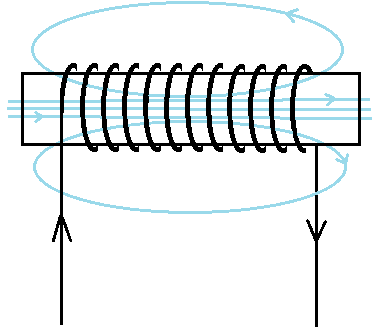
\includegraphics[scale=0.6]{electroaimant.png}
\caption{Modélisation d'un électroaimant}
\label{modélisation de l'électroaimant}
\end{figure}

Le nombre de spires de la bobine fixe, appelons-le $N_1$, a été choisi arbitrairement de manière à produire un
champ magnétique assez fort. Nous avons fixé ce nombre, selon les conseils de notre tuteur, à \numprint{420}. 
Nous allons maintenant calculer les caractéristiques suivantes de notre électroaimant :

\begin{itemize}
	\item Résistance totale de la bobine ;
	\item Champ magnétique induit ;
	\item Inductance.
\end{itemize}

\paragraph{Champ magnétique dans l'entrefer}
Pour céer un champ magnétique plus fort, nous avons réduit l'entrefer de $\unit{7}{\milli\meter}$.
Calculons dans un premier temps le champ magnétique dans l'entrefer de $\unit{7}{\milli\meter}$ en 
utilisant la conservation des flux. Pour ce calcul, nous utilisons l'hypothèse simplificatrice
assez forte que tout le champ se trouve dans l'entrefer.

$$H_e \cdot e = N_1 I \Rightarrow \frac{B_e}{\mu_0 \mu_r} e = N_1 I$$

Pour $N_1 = 420$, l'entrefer $e = \unit{0.007}{\meter}$, $\mu_r = 1.0000004$ la perméabilité magnétique
de l'air et $I = \unit{1}{\ampere}$, on trouve alors :

$B_e = \unit{0.07539825}{\tesla}$

\paragraph{Résistance totale de la bobine}
Pour calculer la résistance totale de la bobine, nous devons connaître la longueur totale de fil de cuivre utilisé.
Pour cela nous utilisons la formule suivante :

$$L{fil} = N_1 \cdot 2\pi r$$  

Où $N_1 = 420$ est le nombre de spires de la bobine fixe, et $r$ est la rayon des spires. Pour
$r = \unit{0.016}{\meter}$, on trouve :

$$L_{fil} = \unit{42.22}{\meter}$$

Il ne nous reste donc plus qu'à multiplier la longueur totale trouvée par la résistance linéique des fils de cuivre
($R_{lin} = \unit{0.18}{\ohm\per\meter}$) :

$$R = L_{fil} \cdot R_{lin} = \unit{7.6}{\ohm}$$

\paragraph{Inductance de la bobine}
Une fois le champ magnétique induit connu, l'inductance dans la bobine peut être très facilement calculée par :

$$L = N_1 \frac{\phi_B}{I}$$

Dans cette formule, il ne nous reste plus qu'à calculer $\phi_B = B \cdot A$ où $A = ab$ est l'aire d'une spire.
On trouve alors :

$L = \unit{0.025468}{\henry}$

\paragraph{Tableau récapitulatif}

\begin{center}
	\begin{tabular}{c|c|c|c|c}
		$N_1$ & $B_e$ & $R$ & $L$ & $L_{fil}$ \\
		\hline
		420 & $\unit{0.07539825}{\tesla}$ & \unit{7.6}{\ohm} & $\unit{0.0254683}{\henry}$ & $\unit{42.22}{\meter}$\\
	\end{tabular}
\end{center}

%Il faut encore recalculer la constante de raideur de la menbranne!

\subsection{Calcul de la constante de raideur de la membrane}
Avant de pouvoir déterminer le nombre de spires de la bobine mouvante, nous avons dû déterminer
expérimentalement la constante de raideur de notre papier pour faire la membrane.
Notre procédure a été la suivante: nous avons suspendu notre membrane, pour ensuite 
déposer un poids dessus, et finalement mesurer l'élongation du matériau.
Nous obtenons ainsi une constante de raideur d'environ \unit {80}{N/m}.

\subsection{Fonctionnement et dimensionnement de la bobine mobile}

\paragraph{Calcul du nombre de spires}
Etant donné que nous disposons d'un amplificateur qui, selon la datasheet, a une puissance de sortie de 
$\unit{2.5}{\watt}$, et que la tension de sortie est de $\unit{15}{\volt}$, nous pouvons trouver le courant
maximal passant dans la bobine mobile:

$$I = \frac{P}{V} = \unit{0.1667}{\ampere}$$

En fonction de la constante de raideur de la membrane trouvée dans la sous-section précédente et de l'écartement
maximal de la membrane par rapport à sa position d'origine (fixé à $d = \unit{0.003}{\meter}$), nous sommes en
mesure de trouver la longueur du fil de la bobine:

$$IL_{fil}B = kx$$
$$L_{fil} = \frac{kx}{IB} = 12.6 m$$

Le fil à notre disposition au laboratoire a un encombrement de $\unit{25.8}{\frac{spires}{cm}}$. Nous otenons 
donc une relation entre $N_2$, le nombre de spires, et $L_{bobine}$, la longueur de la bobine:

$$25.8 = \frac{N_2}{L_{bobine}}$$

En fixant le rayon à \unit{1.7}{mm}, nous pouvons déterminer $N_2$ ainsi que la longueur de la bobine:
$$L_{fil} = N_2 \cdot 2\pi r$$ 
$$N_2 =  \frac{L_{fil}}{2\pi r} = 118$$


\paragraph{Calcul de la résistance totale de la bobine mobile}
Pour calculer la résistance totale de la bobine, il ne nous reste plus qu'à multiplier la longueur de fil trouvée 
précédemment par la résistance linéique du fil de cuivre
($R_{lin} = \unit{0.18}{\ohm\per\meter}$) :

$$R = L_{fil} \cdot R_{lin} = \unit{2.38}{\ohm}$$

\paragraph{Calcul de l'inductance de la bobine mobile}

Une fois le champ magnétique induit connu, l'inductance dans la bobine peut être très facilement calculée par :

$$L = N_2 \frac{\phi_B}{I} = \unit{0.0734}{\henry}$$

\paragraph{Tableau récapitulatif}

\begin{center}
	\begin{tabular}{c|c|c|c}
		$N_2$ & $I$ & $R$ & $L$ \\
		\hline
		 $118$ & $\unit{0.1667}{\ampere}$ & $\unit{2.38}{\ohm}$ & $\unit{0.0734}{\henry}$ \\
	\end{tabular}
\end{center}

\begin{figure}[ht!]
\centering
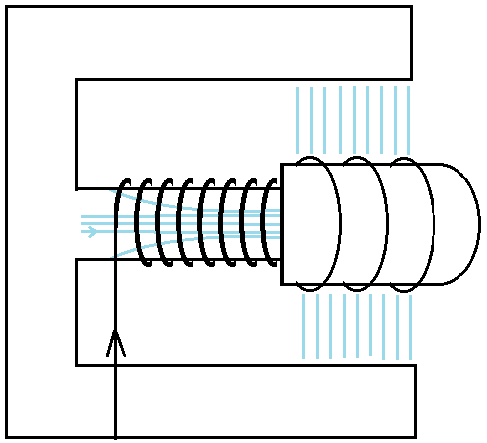
\includegraphics[scale=0.3]{hautparleur.png}
\caption{Vue d'ensemble avec la seconde bobine}
\label{Vue d'ensemble avec la seconde bobine}
\end{figure}

% Just here to fix rapport_prejury.tex
\end{document}
\clearpage

% A terminer avant de mettre dans le rapport, sinon tant pis (car pas obligatoire)
% \documentclass{article}

\usepackage[utf8]{inputenc}
\usepackage[T1]{fontenc}      
\usepackage[francais]{babel}
\usepackage{graphicx}
\usepackage{circuitikz}
\usepackage[squaren, Gray]{SIunits}
\usepackage{sistyle}
\usepackage[autolanguage]{numprint}
\usepackage{pgfplots}
\pgfplotsset{compat=1.9}
\usepackage{amsmath,amssymb,array}
\usepackage[top=2.5cm,bottom=2.5cm,right=2.5cm,left=2.5cm]{geometry}
\usepackage{url} 
\usepackage{tabularx}
\DeclareMathOperator{\dist}{d}
\newenvironment{abstract-fr}
{
	\begin{center}
		\textbf{Résumé} \\[0.5cm]
	\end{center}
}
{}

\newenvironment{abstract-en}
{
	\begin{center}
		\textbf{Summary} \\[0.5cm]
	\end{center}
}
{}
% New command pour la modélisation mécanique, tri à effectuer
\newcommand\fv[1]{{\bf #1}} % free vector
\newcommand\fvd[1]{\dot{\bf #1}} % free vector derivated
\newcommand\fvdd[1]{\ddot{\bf #1}} % free vector derivated
\newcommand\fvr[1]{\mathring{\bf #1}} % free vector relatively derivated
\newcommand\fvrr[1]{\overset{\circ\circ}{\bf #1}} % free vector relatively derivated
\newcommand\uv[1]{{\bf\hat{ #1}}} % unit vector
\newcommand\ui{{\bf\hat{I}}} % unit vector I
\newcommand\uj{{\bf\hat{J}}} % unit vector J
\newcommand\uk{{\bf\hat{K}}} % unit vector K
\newcommand\wrt[2]{\ensuremath{\tensor*[_{ #1}]{ #2}{}}} % With Respect To
\newcommand\wtr[3]{\ensuremath{\tensor*[_{ #1}]{ #2}{^{ #3}}}} % With Two Respect
\newcommand\omegaf{{\bm \omega}}
\newcommand\omegafr{\mathring{\bm \omega}}
\newcommand\omegafd{\dot{\bm \omega}}
\newcommand\omegaft{\tilde{\bm \omega}}
\newcommand\omegaftr{\mathring{\tilde{\bm \omega}}}
\newcommand\omegat{\tilde{\omega}}
\newcommand\omegatd{\tilde{\dot{\omega}}}
\newcommand\ine{{\bf I}}
\newcommand\st{{\bf L}}
\newcommand\pst{{\bf M}}
\newcommand\lm{{\bf N}}
\newcommand\am{{\bf H}}
\newcommand\amd{\dot{\am}}
\newcommand\fo{{\bf F}}
\newcommand\po{\mathcal{P}}
\newcommand\xg{\ensuremath{\fv{R}}}
\newcommand\xgd{\ensuremath{\fvd{R}}}
\newcommand\xgdd{\ensuremath{\fvdd{R}}}
\newcommand\dvec[1]{\dot{\vec{ #1}}}
\newcommand\ddvec[1]{\ddot{\vec{ #1}}}
\newcommand\qp{\dot{q}}
\newcommand\dqp{\Delta \dot{q}}
\usepackage{url} 
\usepackage{hyperref}
\hypersetup{
    colorlinks,
    citecolor=black,
    filecolor=black,
    linkcolor=black,
    urlcolor=black
}

\begin{document}

\section{Modélisation mécanique du haut-parleur}

\subsection{Composition du haut-parleur}
Le haut-parleur est constitué de différentes parties : une membrane
attachée par des fixations qui jouent le rôle de ressorts et reliée à 
une bobine mobile et une bobine fixe qui s'emboîte (sans frottement) 
dans cette dernière.

La bobine fixe va permettre à la bobine mobile de se déplacer exclusivement de gauche
à droite (voir Figure \ref{hp-scheme}), permettant ainsi à la membrane de vibrer 
(et donc de produire un son). Tout déplacement dans une autre direction serait dommageable
car risquerait d'abîmer la membrane.

\begin{figure}[ht!]
	\centering
	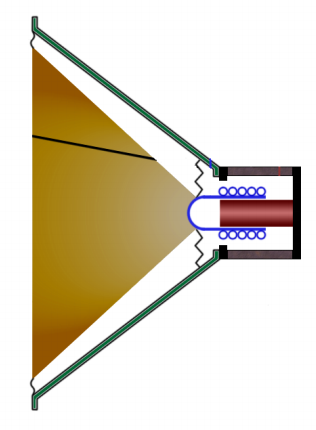
\includegraphics[scale=0.6]{haut-parleur.png}
	\caption{Schéma d'un haut-parleur. (Source : \textit{Modélisation mécanique du haut-parleur} sur iCampus)}
	\label{hp-scheme}
\end{figure}

\subsection{Étude du mouvement de la bobine mobile}
Nous allons maintenant écrire les équations du mouvement de la bobine mobile.
Pour ce faire, nous plaçons un repère fixe $\{\ui\}$ dont l'origine $O$ se trouve
au centre de gravité de la bobine mobile à sa position d'équilibre (au 
temps $t=0$). $\uv{I}_1$ est parallèle à la bobine et dirigé vers la gauche, tandis que
$\uv{I}_2$ est dirigée perpendiculairement à la bobine mobile, vers le haut.
La bobine mobile ne possède qu'un seul degré de liberté, qui
est la distance entre $O$ et son centre de gravité; notons-la $\fv{x}(t)$.
La positon de la bobine est donc donnée par :

$$\vec{R(t)} = \fv{x}(t) \uv{I}_1$$ 

\paragraph{Inventaire des forces}
Avant d'écrire l'équation du mouvement de la bobine, établissons l'inventaire
des forces qui agissent sur celle-ci :

\begin{itemize}
	\item Son poids, dont la résultante agit sur son centre de gravité : $-mg\uv{I}_2$ ;
	\item La force de rappel des fixations (que l'on suppose agir comme des simples
	ressorts) : $-k \fv{x}(t) \uv{I}_1$ où $k$ est la constante de raideur des fixations ;
	\item La force électromagnétique causée par l'électroaimant : $BLi(t) \uv{I}_1$ où
	$B$ est le champ magnétique produit par l'électroaimant, $L$ la longueur de fil de cuivre
	utilisé et $i(t)$ le courant électrique ;
	\item Le frottement dû à l'air ;
\end{itemize}

Parmis toute ces forces, nous négligeons le frottement dû à l'air ainsi que le poids
de la bobine mobile (sa masse étant relativement faible).

\paragraph{Équation du mouvement}
Nous avons maintenant tout à notre disposition pour écrire les équations du mouvement
\footnote{Dans cette section, nous utilisons les notations employées au cours de
mécanique des corps rigides.} :

$$m\fvdd{x}(t) = -k\fv{x}(t) + BLi(t)$$

En sachant que le signal d'entrée est une fonction de la forme $V(t) = V_0 \cos (\omega t)$ et
que, par la loi d'Ohm, $V(t) = Ri(t)$ où $R$ est la résistance du circuit, 
nous pouvons réecrire l'équation différentielle du mouvement de la manière suivante :

$$m\fvdd{x}(t) + k\fv{x}(t) = \frac{B2\pi rNV_0}{R}\cos (\omega t)$$

Où nous avons également fait apparaître le nombre de spires $N$ et le rayon de la bobine
$r$. Il ne reste donc plus qu'à résoudre cette équation différentielle.

\paragraph{Résolution de l'équation différentielle du mouvement}
Résolvons cette équation différentielle comme appris lors de ce deuxième
quadrimestre. Cherchons d'abord la solution homogène de cette équation, notée $\fv{x}_h(t)$.
Pour ce faire, résolvons le polynôme caractéristique :

$$mr^2 + k = 0 \Rightarrow r = \pm i\sqrt{\frac{k}{m}}$$

Nous avons donc, en ne gardant que la partie réelle :

$$\fv{x}_h(t) = Ae^{i\sqrt{\frac{k}{m}}t} + Be^{-i\sqrt{\frac{k}{m}}}$$

Où $A$ et $B$ sont des coéfficients complexes. Nous pouvons réecrire cette solution
en termes de fonctions trigonométriques. En ne gardant que la partie réelle, 
nous obtenons :

$$\fv{x}_h(t) = C\cos(\sqrt{\frac{k}{m}}t) - D\sin(\sqrt{\frac{k}{m}}t)$$

Où $C$ et $D$ sont cette-fois des coefficients réels.

Penchons-nous maintenant sur la solution particulière, notée $\fv{x}_p(t)$. Pour
cette partie de la résolution, nous réécrivons le terme non-homogène sous la forme d'une
exponentielle complexe. La solution particulière est de la forme :

$$\fv{x}_p(t) = \alpha e^{\omega it}}$$

En injectant $\fv{x}_p(t)$ et sa dérivée seconde dans l'équation de départ, nous trouvons :

$$\alpha = \frac{2\pi rNV_0}{R(-m\omega^2 + k)} \Rightarrow \fv{x}_p(t) = \frac{2\pi rNV_0}{R(-m\omega^2 + k)}e^{wit}$$

En ne gardant que la partie réelle de l'exponentielle, nous avons finalement :

$$\fv{x}_p(t) = \frac{2\pi rNV_0}{R(-m\omega^2 + k)} \cos (\omega t)$$

Par le principe de superposition des solutions des équations différentielles :

$$\fv{x}(t) = \fv{x}_h(t) + \fv{x}_p(t) = C\cos(\sqrt{\frac{k}{m}}t) - D\sin(\sqrt{\frac{k}{m}}t) + \frac{2\pi rNV_0}{R(-m\omega^2 + k)} \cos (\omega t)$$

En utilisant la première condition initiale, $\fv{x}(0) = 0$, nous trouvons:

$$C = \frac{-BLV_0}{R(-m\omega^2+k}$$

Il reste à trouver une deuxième condition initiale.

\subsection{Fréquence de résonance}
Nous remarquons que si $\omega \rightarrow \sqrt{\frac{k}{m}}$, le dénominateur de l'amplitude du mouvement
tend vers \numprint{0}, et donc l'amplitude du mouvement tend vers $\infty$. Cette situation n'a physiquement
pas de sens. Nous notons cette fréquence $\omega_0$; il s'agit de la \textit{fréquence de résonance}.

\subsection{Couplage entre mouvement et son émis}
Étudions maintenant le mouvement de la deuxième couche
d'air representée sur la Figure \ref{wave-sound-scheme}.
La couche numérotée \numprint{0} représente la membrane.
La pression dans la couche d'air numérotée \numprint{1} 
est $p_0 + dp(t)$. Dans les couches suivantes, elle est
constante vaut $P_0$. Nous considérons un problème simplifié
à une dimension (déplacement de tranche d'air dans un
tuyau). Nous prenons également l'hypothèse que les couches
d'air sont incompressibles afin de pouvoir appliquer
ce que nous avons appris au cours de mécanique des corps
rigides.

Plaçons le repère inertiel ${\ui}$ tel que $\uv{I}_1$
est orienté vers la droite horizontalement et $\uv{I}_2$
orienté vers le haut verticalement. Plaçons l'origine
$O$ de ce repère à la position initiale de la couche
d'air. La position de la couche d'air, notée $\vec{R(t)}$ vaut 
donc :

$$\vec{R(t)} = \fv{x}(t)\uv{I}_1$$

\begin{figure}[ht!]
	\centering
	\includegraphics[scale=0.6]{onde-sonore.png}
	\caption{Déplacement de tranche de couche d'air dans un tuyau. (Source : \textit{Modélisation mécanique du haut-parleur} sur iCampus)}
	\label{wave-sound-scheme}
\end{figure}

\paragraph{Inventaire des forces}
Comme pour la bobine mobile, faisons l'inventaire
des forces qui s'exercent sur la deuxième couche d'air :

\begin{itemize}
	\item Le poids de la couche d'air : $-\rho A\uv{I}_2$, ou $\rho$ est la densité volumique
	de l'air et $A$ est la surface de la couche d'air ;
	\item La pression exercée sur la couche \numprint{2} par la pression dans la couche \numprint{1}
	: $(p_0 + dp(t))A \uv{I}_1$.
\end{itemize}

\paragraph{Équation du mouvement}
Nous pouvons maintenant écrire l'équation du mouvement

% Just here to fix rapport_prejury.tex
\end{document}

% \clearpage

\documentclass{article}

\usepackage[utf8]{inputenc}
\usepackage[T1]{fontenc}      
\usepackage[francais]{babel}
\usepackage{graphicx}
\usepackage{circuitikz}
\usepackage[squaren, Gray]{SIunits}
\usepackage{sistyle}
\usepackage[autolanguage]{numprint}
\usepackage{pgfplots}
\pgfplotsset{compat=1.9}
\usepackage{amsmath,amssymb,array}
\usepackage[top=2.5cm,bottom=2.5cm,right=2.5cm,left=2.5cm]{geometry}
\usepackage{url} 
\usepackage{tabularx}
\DeclareMathOperator{\dist}{d}
\newenvironment{abstract-fr}
{
	\begin{center}
		\textbf{Résumé} \\[0.5cm]
	\end{center}
}
{}

\newenvironment{abstract-en}
{
	\begin{center}
		\textbf{Summary} \\[0.5cm]
	\end{center}
}
{}
% New command pour la modélisation mécanique, tri à effectuer
\newcommand\fv[1]{{\bf #1}} % free vector
\newcommand\fvd[1]{\dot{\bf #1}} % free vector derivated
\newcommand\fvdd[1]{\ddot{\bf #1}} % free vector derivated
\newcommand\fvr[1]{\mathring{\bf #1}} % free vector relatively derivated
\newcommand\fvrr[1]{\overset{\circ\circ}{\bf #1}} % free vector relatively derivated
\newcommand\uv[1]{{\bf\hat{ #1}}} % unit vector
\newcommand\ui{{\bf\hat{I}}} % unit vector I
\newcommand\uj{{\bf\hat{J}}} % unit vector J
\newcommand\uk{{\bf\hat{K}}} % unit vector K
\newcommand\wrt[2]{\ensuremath{\tensor*[_{ #1}]{ #2}{}}} % With Respect To
\newcommand\wtr[3]{\ensuremath{\tensor*[_{ #1}]{ #2}{^{ #3}}}} % With Two Respect
\newcommand\omegaf{{\bm \omega}}
\newcommand\omegafr{\mathring{\bm \omega}}
\newcommand\omegafd{\dot{\bm \omega}}
\newcommand\omegaft{\tilde{\bm \omega}}
\newcommand\omegaftr{\mathring{\tilde{\bm \omega}}}
\newcommand\omegat{\tilde{\omega}}
\newcommand\omegatd{\tilde{\dot{\omega}}}
\newcommand\ine{{\bf I}}
\newcommand\st{{\bf L}}
\newcommand\pst{{\bf M}}
\newcommand\lm{{\bf N}}
\newcommand\am{{\bf H}}
\newcommand\amd{\dot{\am}}
\newcommand\fo{{\bf F}}
\newcommand\po{\mathcal{P}}
\newcommand\xg{\ensuremath{\fv{R}}}
\newcommand\xgd{\ensuremath{\fvd{R}}}
\newcommand\xgdd{\ensuremath{\fvdd{R}}}
\newcommand\dvec[1]{\dot{\vec{ #1}}}
\newcommand\ddvec[1]{\ddot{\vec{ #1}}}
\newcommand\qp{\dot{q}}
\newcommand\dqp{\Delta \dot{q}}
\usepackage{url} 
\usepackage{hyperref}
\hypersetup{
    colorlinks,
    citecolor=black,
    filecolor=black,
    linkcolor=black,
    urlcolor=black
}

\begin{document}

\section{Dimensionnement du haut-parleur}
Après avoir réalisé quelques recherches sur les haut-parleurs, nous avons pu imaginer le dispositif idéal 
à réaliser. En tenant compte des différentes contraintes qui nous étaient imposées, voici les différents 
choix que nous avons effectués.

\subsection{Pour le boîtier}
Nous devions pouvoir faire varier les fréquences (voir annexe "Cahier des Charges"), ce qui signifie que nous ne 
pouvions pas faire un caisson trop petit. La taille du caisson influence le son restitué par le haut-parleur :
un volume trop petit ne restituerait pas les extrêmes graves. Effectivement, à de très basses 
fréquences, l'enceinte close va se comporter comme une raideur supplémentaire qui augmente la fréquence de
résonance\footnote{Fréquence pour laquelle la réponse du circuit est maximale}, et donc augmente la 
fréquence de coupure du passe-haut\cite{volume}. Nous avons finalement opté pour un boîtier cubique de 
$\unit{25}{\centi\meter}$ de côté, étant donné que ces dimensions avaient eu un très beau résultat lors 
d'un projet d'une année antérieure. Nous avions pensé placer un évent à l'avant du haut-parleur 
pour augmenter le rendement en profitant de l'onde arrière, mais c'était plus difficile à construire, et 
il aurait fallu que l'on accorde l'évent, de manière à exploiter l'onde arrière correctement. Nous nous 
sommes donc finalement limités à une charge\footnote{Manière de séparer les ondes avant et arrière.} dite "\textit{close}"\cite{close}.  

Afin d'améliorer un peu le boîtier, nous avons également pensé aux éléments suivants :

\begin{itemize}
	\item	Des pieds en caoutchouc : placer des pieds en caoutchouc sur le boîtier de notre haut-parleur
				permet de réduire les déplacements dûs aux vibrations du haut-parleur ;
	\item	Un matériau acoustiquement absorbant à l'intérieur du haut-parleur : le but d'un tel matériau
				dans un haut-parleur est de supprimer le court-circuit acoustique\cite{absorber}.
\end{itemize}

\subsection{Pour la membrane}
Nous avons opté pour une membrane de diamètre de $\unit{17}{\centi\meter}$. Nous avons choisi cette valeur afin 
d'avoir une membrane assez large, pour exploiter le mieux possible la taille du caisson. C'est également un
diamètre assez répandu dans le commerce\cite{tlhp}. Nous respectons donc les normes.
La profondeur de la membrane est de $\unit{6}{\centi\meter}$, comme pour la plupart des membranes de ce
diamètre\cite{tlhp}. La membrane est réalisée en papier. Afin d'éviter les difficultés de pliage, nous avons opté pour
du tissus tendu en guise de ressort. 

\begin{table}[!htb]
	\centering
	\begin{tabularx}{\textwidth}{|X|X|}
		\hline
			 \textbf{Caractéristique} & \textbf{Justification} \\
		\hline
			Volume du caisson : $\unit{25\times25\times25}{\centi\meter}$ & Possibilité de faire varier les fréquences.  \\
		\hline
			Matériau du caisson : Panneau de 	MDF
			d'épaisseur \unit{18}{\milli\meter} & Qualité, robustesse et coût. \\
		\hline
			Diamètre de membrane : \unit{17}{\centi\meter} & Avoir une membrane assez large pour exploiter le mieux possible la taille du caisson. \\
		\hline
			Profondeur de la membrane : \unit{6}{\centi\meter} & Déterminé en fonction du diamètre de la membrane. \\
		\hline
			Materiau membrane : papier et tissus & Rigidité et petite constante de raideur. \\
		\hline
			Masse surfacique du papier : \unit{200}{\gram\per\meter\squared} & Rigidité et coût. \\
		\hline
	\end{tabularx}
	\caption{Tableau récapitulatif.}
\end{table}

% Just here to fix rapport_prejury.tex
\end{document}


\chapter{Recherche documentaire}

\documentclass{article}

\usepackage[utf8]{inputenc}
\usepackage[T1]{fontenc}      
\usepackage[francais]{babel}
\usepackage{graphicx}
\usepackage{circuitikz}
\usepackage[squaren, Gray]{SIunits}
\usepackage{sistyle}
\usepackage[autolanguage]{numprint}
\usepackage{pgfplots}
\pgfplotsset{compat=1.9}
\usepackage{amsmath,amssymb,array}
\usepackage[top=2.5cm,bottom=2.5cm,right=2.5cm,left=2.5cm]{geometry}
\usepackage{url} 
\usepackage{tabularx}
\DeclareMathOperator{\dist}{d}
\newenvironment{abstract-fr}
{
	\begin{center}
		\textbf{Résumé} \\[0.5cm]
	\end{center}
}
{}

\newenvironment{abstract-en}
{
	\begin{center}
		\textbf{Summary} \\[0.5cm]
	\end{center}
}
{}
% New command pour la modélisation mécanique, tri à effectuer
\newcommand\fv[1]{{\bf #1}} % free vector
\newcommand\fvd[1]{\dot{\bf #1}} % free vector derivated
\newcommand\fvdd[1]{\ddot{\bf #1}} % free vector derivated
\newcommand\fvr[1]{\mathring{\bf #1}} % free vector relatively derivated
\newcommand\fvrr[1]{\overset{\circ\circ}{\bf #1}} % free vector relatively derivated
\newcommand\uv[1]{{\bf\hat{ #1}}} % unit vector
\newcommand\ui{{\bf\hat{I}}} % unit vector I
\newcommand\uj{{\bf\hat{J}}} % unit vector J
\newcommand\uk{{\bf\hat{K}}} % unit vector K
\newcommand\wrt[2]{\ensuremath{\tensor*[_{ #1}]{ #2}{}}} % With Respect To
\newcommand\wtr[3]{\ensuremath{\tensor*[_{ #1}]{ #2}{^{ #3}}}} % With Two Respect
\newcommand\omegaf{{\bm \omega}}
\newcommand\omegafr{\mathring{\bm \omega}}
\newcommand\omegafd{\dot{\bm \omega}}
\newcommand\omegaft{\tilde{\bm \omega}}
\newcommand\omegaftr{\mathring{\tilde{\bm \omega}}}
\newcommand\omegat{\tilde{\omega}}
\newcommand\omegatd{\tilde{\dot{\omega}}}
\newcommand\ine{{\bf I}}
\newcommand\st{{\bf L}}
\newcommand\pst{{\bf M}}
\newcommand\lm{{\bf N}}
\newcommand\am{{\bf H}}
\newcommand\amd{\dot{\am}}
\newcommand\fo{{\bf F}}
\newcommand\po{\mathcal{P}}
\newcommand\xg{\ensuremath{\fv{R}}}
\newcommand\xgd{\ensuremath{\fvd{R}}}
\newcommand\xgdd{\ensuremath{\fvdd{R}}}
\newcommand\dvec[1]{\dot{\vec{ #1}}}
\newcommand\ddvec[1]{\ddot{\vec{ #1}}}
\newcommand\qp{\dot{q}}
\newcommand\dqp{\Delta \dot{q}}
\usepackage{url} 
\usepackage{hyperref}
\hypersetup{
    colorlinks,
    citecolor=black,
    filecolor=black,
    linkcolor=black,
    urlcolor=black
}

\begin{document}

\section{La contre-réaction ou réaction négative}
En analysant le circuit de notre haut-parleur, nous avons découvert la présence de boucle reliant la sortie et la borne négative des amplificateurs. Nous nous sommes alors interrogés sur le rôle de ces boucles.

Nous allons dans un premier temps expliquer les raisons d'être des boucles de contre-réaction en général et nous finirons par l'explication complète de leur raison d'être dans le cas particulier de notre circuit.

\subsection{Principe de la réaction}
Le principe de la réaction est présent dans un grand nombre de circuits électroniques. Il consiste en une réinjection d'une partie du signal de sortie à l'entrée du circuit pour le combiner avec le signal d'entrée extérieur.

Il existe deux types de réactions :

\begin{itemize}
	\item \textbf{La réaction positive} : le signal réinjecté est en phase avec le signal d'entrée de telle sorte que les deux signaux s'additionnent ;
	\item \textbf{La réaction négative} (ou contre-réaction) : le signal réinjecté est en opposition de phase avec le signal d'entrée, de telle sorte que les deux signaux
	se soustraient.
\end{itemize}

\begin{figure}[h]
	\centering
	\begin{circuitikz}
		\draw (0, 0) node[ocirc];
		\draw (0, 0)	to[short] (2, 0);
		\draw (0, -1) node[ocirc];
		\draw (0, -1) to[short] (2, -1);
		\draw (3.1, -0.5) node [op amp, yscale=-1.022] (op amp) {}
					(opamp.-)node[left]
					(opamp.+)node[left]
					(opamp.out)node[right];
		\draw (3.85, -0.5) to[short] (5.6, -0.5);
		\draw (5.6, -0.5) node[ocirc];
		\draw (5.4, -0.5) to[short] (5.4, -2);
		\draw (5.4, -2) to[short] (1.4, -2);
		\draw (1.4, -2) to[short] (1.4, -1);
	\end{circuitikz}
	\caption{Schéma électrique d'une boucle de réaction sur un 	amplificateur.}
	\label{reaction1}
\end{figure}

\subsection{Effets des boucles de contre-réaction}

\subsubsection{En général}
Les effets des boucles de contre-réaction sur un amplificateur sont nombreux :

\begin{itemize}
	\item La boucle de contre-réaction rend indépendant le gain de l'amplificateur des différentes variations du circuits ;
	\item Le signal de sortie est plus proche du signal d'entrée que si l'amplificateur avait été en boucle ouverte ;
	\item Réduction des signaux électriques parasites et de la distorsion dûs à l'amplificateur : en boucle ouverte, le taux de distorsion d'un amplificateur est typiquement de 1\%. La boucle de contre-réaction permet de diminuer ce taux à 0.001\% ;
	\item Contrôle du gain de l'amplificateur (qui est, en boucle ouverte, de l'ordre de $10^6$) ;
	\item Elargissement de la bande passante de l'amplificateur ;
	\item Réduction de l'impédance de sortie.
\end{itemize}

\subsubsection{Dans notre cas particulier}
Dans notre cas particulier, le principal effet de la boucle de contre-réaction est le contrôle du gain de l'amplificateur qui ramène à $1$ le gain.

\begin{figure}[h]
	\centering
	\begin{circuitikz}
		\draw (0,0) node[ocirc];
		\draw (3,0) to[short] (opamp+);
		\draw (4, -0.5) node [op amp, yscale=-1.022] (op amp) {}
			(opamp.-)node[left] (opamp-)
			(opamp.+)node[left] (opamp+)
			(opamp.out)node[right] (opampout);
		\draw (5, -0.5) to[short] (7, -0.5);
		\draw (7, -0.5) node[ocirc];
		\draw (2, -1) to[short] (3, -1);
		\draw (2, -1) to[short] (2, -3);
		\draw (2, -3) to[R=$R_1$] (2, -4);
		\draw (2, -4) to[short] (2, -4.5);
		\draw (2, -4) node[ground];
		\draw (2, -2) to[short] (6, -2);
		\draw (6, -2) to[R=$R_2$] (6, -0.5);
	\end{circuitikz}
	\caption{Schéma électrique d'une boucle de réaction sur un 	amplificateur avec un diviseur résistif.}
	\label{reaction2}
\end{figure}

Sur la Figure \ref{reaction2}, on remarque que la tension de sortie et la tension d'entrée sont liées par la formule des diviseurs résistifs :

$$V_{in} = \frac{R_1}{R_1 + R_2} V_{out}$$

Le gain est alors donné par :

$$A = \frac{V_{out}}{V_{in}} = \frac{R_1 + R_2}{R_1}$$

Pour réduire le gain $A$ à $1$, on a alors deux possibilités :

\begin{enumerate}
	\item	Choisir $R_1 >> R_2$ ;
	\item Choisir $R_2 = 0$ ;
\end{enumerate}

La possibilité la plus simple est la deuxième, car en choississant $R_2 = 0$, le gain est donné par $\frac{R_1}{R_1}$. Autrement dit : quelque soit $R_1$, on a $A = 1$ de telle sorte que $V_{in} = V_{out}$. On choisi alors $R_1$ si petit que le remplacer par un simple court-circuit a le même effet.

Dans un tel montage (appelé \texit{suiveur de tension}), la résistance d'entrée est infinie alors que la résistance de sortie est faible. Le courant de sortie est alors plus grand que le courant d'entrée (qui est presque nul).

\nocite{*} 
\bibliographystyle{plain}
\bibliography{source}

% Just here to fix rapport_prejury.tex
\end{document}
\clearpage

\documentclass{article}

\usepackage[utf8]{inputenc}
\usepackage[T1]{fontenc}      
\usepackage[francais]{babel}
\usepackage{graphicx}
\usepackage{circuitikz}
\usepackage[squaren, Gray]{SIunits}
\usepackage{sistyle}
\usepackage[autolanguage]{numprint}
\usepackage{pgfplots}
\pgfplotsset{compat=1.9}
\usepackage{amsmath,amssymb,array}
\usepackage[top=2.5cm,bottom=2.5cm,right=2.5cm,left=2.5cm]{geometry}
\usepackage{url} 
\usepackage{tabularx}
\DeclareMathOperator{\dist}{d}
\newenvironment{abstract-fr}
{
	\begin{center}
		\textbf{Résumé} \\[0.5cm]
	\end{center}
}
{}

\newenvironment{abstract-en}
{
	\begin{center}
		\textbf{Summary} \\[0.5cm]
	\end{center}
}
{}
% New command pour la modélisation mécanique, tri à effectuer
\newcommand\fv[1]{{\bf #1}} % free vector
\newcommand\fvd[1]{\dot{\bf #1}} % free vector derivated
\newcommand\fvdd[1]{\ddot{\bf #1}} % free vector derivated
\newcommand\fvr[1]{\mathring{\bf #1}} % free vector relatively derivated
\newcommand\fvrr[1]{\overset{\circ\circ}{\bf #1}} % free vector relatively derivated
\newcommand\uv[1]{{\bf\hat{ #1}}} % unit vector
\newcommand\ui{{\bf\hat{I}}} % unit vector I
\newcommand\uj{{\bf\hat{J}}} % unit vector J
\newcommand\uk{{\bf\hat{K}}} % unit vector K
\newcommand\wrt[2]{\ensuremath{\tensor*[_{ #1}]{ #2}{}}} % With Respect To
\newcommand\wtr[3]{\ensuremath{\tensor*[_{ #1}]{ #2}{^{ #3}}}} % With Two Respect
\newcommand\omegaf{{\bm \omega}}
\newcommand\omegafr{\mathring{\bm \omega}}
\newcommand\omegafd{\dot{\bm \omega}}
\newcommand\omegaft{\tilde{\bm \omega}}
\newcommand\omegaftr{\mathring{\tilde{\bm \omega}}}
\newcommand\omegat{\tilde{\omega}}
\newcommand\omegatd{\tilde{\dot{\omega}}}
\newcommand\ine{{\bf I}}
\newcommand\st{{\bf L}}
\newcommand\pst{{\bf M}}
\newcommand\lm{{\bf N}}
\newcommand\am{{\bf H}}
\newcommand\amd{\dot{\am}}
\newcommand\fo{{\bf F}}
\newcommand\po{\mathcal{P}}
\newcommand\xg{\ensuremath{\fv{R}}}
\newcommand\xgd{\ensuremath{\fvd{R}}}
\newcommand\xgdd{\ensuremath{\fvdd{R}}}
\newcommand\dvec[1]{\dot{\vec{ #1}}}
\newcommand\ddvec[1]{\ddot{\vec{ #1}}}
\newcommand\qp{\dot{q}}
\newcommand\dqp{\Delta \dot{q}}
\usepackage{url} 
\usepackage{hyperref}
\hypersetup{
    colorlinks,
    citecolor=black,
    filecolor=black,
    linkcolor=black,
    urlcolor=black
}

\begin{document}

\section{La distorsion harmonique}

La distorsion est un critère de qualité en ce qui concerne les haut-parleurs.
Dans le soucis de construire un dispositif de qualité, nous avons décidé de 
nous informer sur la distorsion harmonique, un concept que nous ne connaissions
que de nom.
Ce document est structuré comme suit: nous parlerons tout d'abord de la notion  de distorsion 
en général pour ensuite aborder la notion  de distorsion 
harmonique, et finalement décrire ses causes, ses effets,
et les moyens de diminution.

\subsection{Définition}
Commençons tout d'abord par comprendre la notion de distorsion du son: par définition, c'est
une transformation du signal audio par rapport à celui de sortie. Une distorsion n'est généralement pas vraiment souhaitée, étant donné
que le signal en est déformé. Cependant, certains audiophiles en tirent avantage, vu que que quelques
transformations peuvent mener à un son plus chaud et agréable.

\paragraph{La distorsion harnomique}
La distorsion harmonique joue sur la superposition de différentes fréquences:
la fréquence fondamentale et ses harmoniques. Un haut-parleur parfait émettrait seulement la fréquence fondamentale, sans les harmoniques, qui sont donc des "parasites".
On parle d'harmonique pour désigner les multiples entiers de la fréquence fondamentale.
Par exemple, la seconde harmonique d'une fréquence de 50 Hz vaut 100Hz, la troisième 150Hz, etc. La figure 
ci-dessous illustre adéquatement cette notion.
Les harmoniques paires sont les moins incommodantes, étant donné qu'elles représentent la même note, mais à quelques octaves de différence.
Les harmoniques impaires, elles, sont plus gênantes étant donné que la note est différente.

\begin{figure}[h]
\centering
\includegraphics[scale=0.6]{image2.png}
\caption{Superposition d'une fréquence fondamentale et de ses premières hamoniques.}
\label{Superposition d'une fréquence fondamentale et de ses premières hamoniques.}
\end{figure}

\subsection{Causes}
À cause de la distorsion harmonique, le signal que nous faisons circuler dans notre haut-parleur n'est pas
une sinusoïdale parfaite mais plutôt une série de Fourier, c'est-à-dire une somme de sinusoïdes de 
fréquence et d'amplitude différentes. C'est l'appareil en lui-même qui crée la distorsion, étant donné 
qu'il ne reproduit généralement pas parfaitement le signal d'entrée. 
Les charges non-linéaires sont les principales causes de distorsion harmonique. Celles-ci causent 
l'apparition des courants harmoniques qui sont eux-mêmes responsables de la distorsion harmonique.

\subsection{Conséquences}
La distorsion harmonique a plusieurs conséquences néfastes.
La plus importante de toutes vient du fait que les harmoniques impaires génèrent un son dur, et peu agréable. De plus, la distorsion cause un accroissement 
du courant dans un système. Il va en résulter une surchauffe des composantes électriques (conducteurs, 
capacités,...). À la longue, des disfonctionnements non souhaités peuvent provoquer un vieillissement 
précoce du circuit électrique. Il existe de nombreuses autres conséquences néfastes, mais n'oublions pas de préciser que certaines personnes recherchent tout de même ces distorsions pour produire un son plus agréable, au moyen d'harmoniques paires.

\subsection{Solutions}
Pour éviter toute distorsion, ou tout simplement pour émettre un son plus pur et exact, 
il existe différentes solutions. Nous parlerons seulement des filtres actifs 
mais il est intéressant de savoir que d'autre moyens tels que les selfs AC ou DC, ainsi que les redresseurs
multi-pulses, existent. 
Les filtres actifs permettent d'éliminer les harmoniques perturbatrices en injectant des courants
harmoniques de mêmes fréquences mais déphasés d'une demi-période. Cela cause des interférences
destructrices avec les harmoniques dont on souhaite se débarrasser. La résultante est une droite constante
nulle n'influençant pas notre signal.

\nocite{*}
\bibliographystyle{plain}
\bibliography{source}

% Just here to fix rapport_prejury.tex
\end{document}

\chapter{Validation du haut-parleur}

\documentclass{article}

\usepackage[utf8]{inputenc}
\usepackage[T1]{fontenc}      
\usepackage[francais]{babel}
\usepackage{graphicx}
\usepackage{circuitikz}
\usepackage[squaren, Gray]{SIunits}
\usepackage{sistyle}
\usepackage[autolanguage]{numprint}
\usepackage{pgfplots}
\pgfplotsset{compat=1.9}
\usepackage{amsmath,amssymb,array}
\usepackage[top=2.5cm,bottom=2.5cm,right=2.5cm,left=2.5cm]{geometry}
\usepackage{url} 
\usepackage{tabularx}
\DeclareMathOperator{\dist}{d}
\newenvironment{abstract-fr}
{
	\begin{center}
		\textbf{Résumé} \\[0.5cm]
	\end{center}
}
{}

\newenvironment{abstract-en}
{
	\begin{center}
		\textbf{Summary} \\[0.5cm]
	\end{center}
}
{}
% New command pour la modélisation mécanique, tri à effectuer
\newcommand\fv[1]{{\bf #1}} % free vector
\newcommand\fvd[1]{\dot{\bf #1}} % free vector derivated
\newcommand\fvdd[1]{\ddot{\bf #1}} % free vector derivated
\newcommand\fvr[1]{\mathring{\bf #1}} % free vector relatively derivated
\newcommand\fvrr[1]{\overset{\circ\circ}{\bf #1}} % free vector relatively derivated
\newcommand\uv[1]{{\bf\hat{ #1}}} % unit vector
\newcommand\ui{{\bf\hat{I}}} % unit vector I
\newcommand\uj{{\bf\hat{J}}} % unit vector J
\newcommand\uk{{\bf\hat{K}}} % unit vector K
\newcommand\wrt[2]{\ensuremath{\tensor*[_{ #1}]{ #2}{}}} % With Respect To
\newcommand\wtr[3]{\ensuremath{\tensor*[_{ #1}]{ #2}{^{ #3}}}} % With Two Respect
\newcommand\omegaf{{\bm \omega}}
\newcommand\omegafr{\mathring{\bm \omega}}
\newcommand\omegafd{\dot{\bm \omega}}
\newcommand\omegaft{\tilde{\bm \omega}}
\newcommand\omegaftr{\mathring{\tilde{\bm \omega}}}
\newcommand\omegat{\tilde{\omega}}
\newcommand\omegatd{\tilde{\dot{\omega}}}
\newcommand\ine{{\bf I}}
\newcommand\st{{\bf L}}
\newcommand\pst{{\bf M}}
\newcommand\lm{{\bf N}}
\newcommand\am{{\bf H}}
\newcommand\amd{\dot{\am}}
\newcommand\fo{{\bf F}}
\newcommand\po{\mathcal{P}}
\newcommand\xg{\ensuremath{\fv{R}}}
\newcommand\xgd{\ensuremath{\fvd{R}}}
\newcommand\xgdd{\ensuremath{\fvdd{R}}}
\newcommand\dvec[1]{\dot{\vec{ #1}}}
\newcommand\ddvec[1]{\ddot{\vec{ #1}}}
\newcommand\qp{\dot{q}}
\newcommand\dqp{\Delta \dot{q}}
\usepackage{url} 
\usepackage{hyperref}
\hypersetup{
    colorlinks,
    citecolor=black,
    filecolor=black,
    linkcolor=black,
    urlcolor=black
}

\begin{document}

% La description de l’appareillage de mesure est claire et complète
\section{Description de l'appareillage}
Afin de tester le circuit de notre haut-parleur, nous avions besoin d'une alimentation
capable de fournir du $\unit{\pm 15}{\volt}$ (pour alimenter le dual ampli-op ainsi
que l'amplificateur audio). Nous avions donc besoin de deux alimentations DC Topward 
\numprint{3303} DS présentes au laboratoire. Pour obtenir une tension négative par 
rapport à une tension de référence, il faut connecter ensemble les deux chassis,
et les bornes $+$ de la première source, et $-$ de la deuxième source. La première règle
alors la tension négative et la deuxième la tension positive\cite{dctopward}.
Au niveau de l'intensité du courant, étant donné que la puissance maximale de l'amplificateur
audio est de \unit{2.5}{\watt}\cite{datasheetampli} et que la tension d'alimentation est de \unit{15}{\volt}, par
la formule $P = VI$ en utilisant la valeur RMS, on obient \unit{0.23}{\ampere}. Nous règlons
donc les deux sources sur cette valeur. Les câbles des deux alimentations sont ensuite connectés 
au bornier de la plaquette. La sortie de la plaquette est quant à elle reliée à la bobine mobile.

L'électroaimant est lui alimenté en courant continu par une troisième source qui 
fourni un courant de \unit{1}{\ampere}. Le courant maximum supportable par les fils de 
cuivre dont nous disposons étant de \unit{2}{\ampere}\cite{norme-cuivre}, nous prenons
une bonne marge de sécurité afin d'éviter la surchauffe des fils.

Enfin, pour les différentes mesures, nous utilisons :

\begin{itemize}
	\item Un oscilloscope lorsque nous désirons visualiser le signal passant par un point de notre circuit ;
	\item Un multimètre pour mesurer un courant, une tension ou une résistane ;
	\item Un teslamètre pour mesurer l'intensité du champ magnétique produit par notre électroaimant.
\end{itemize}

\section{Compte-rendu des mesures}

\subsection{Mesures du champ magnétique produit par l'électroaimant}
Pour mesurer le champ magnétique produit par l'électroaimant, nous nous servons du teslamètre.
Le champ qui nous intéresse se situe dans l'entrefer de l'électroaimant, il suffit alors de placer
la sonde du teslamètre dans cet entrefer. Il est difficile d'obtenir une mesure très précise en se
servant du teslamètre car la valeur qu'il nous indique n'est pas très stable. Cependant, en répétant
plusieurs fois l'expérience et en notant les valeurs affichées par le teslamètre, nous obtenons une mesure
moyenne de \unit{8}{\centi\tesla} ; un résultat qui confirme nos prédictions théoriques
qui annonçaient un champ magnétique de \unit{7.54}{\centi\tesla}.

\subsection{Mesures en différents points du circuit}
Pour mesurer la tension du signal audio en différents points du circuit, nous utilisons l'oscilloscope
et sa sonde.

\paragraph{Point d'entrée}
Nous avons commencé par mesurer la tension du signal audio sortant de la prise jack. Pour ce faire nous avons
placé la sonde de l'oscilloscope au point IN1 du circuit. Nous avons alors pu visualiser le 
signal audio, comme le montre la figure \ref{in1}.

\begin{figure}[!htb]
	\centering
	\includegraphics[scale=0.15]{IN1.jpg}
	\caption{Signal audio visualisé au point IN1 du circuit.}
	\label{in1}
\end{figure}

En prenant une échelle appropriée, c'est-à-dire \unit{50}{\milli\volt}, on voit que le signal 
audio a une amplitude de \unit{0.0375}{\volt} à la sortie de la prise jack.

\paragraph{Règlage du volume et filtres}

% Je ne parviens pas à exploiter les photos et mesures prises...

\paragraph{Point de sortie}
Au point de sortie, nous avons mesuré une tension située entre \unit{3}{\volt}
et \unit{0.22}{\volt} selon que le potentiomètre lié au réglage du volume
soit sur sa valeur maximale ou sur sa valeur minimale.


% Just here to fix rapport_prejury.tex
\end{document}


\chapter{Conclusion}

\documentclass{article}

\usepackage[utf8]{inputenc}
\usepackage[T1]{fontenc}      
\usepackage[francais]{babel}
\usepackage{graphicx}
\usepackage{circuitikz}
\usepackage[squaren, Gray]{SIunits}
\usepackage{sistyle}
\usepackage[autolanguage]{numprint}
\usepackage{pgfplots}
\pgfplotsset{compat=1.9}
\usepackage{amsmath,amssymb,array}
\usepackage[top=2.5cm,bottom=2.5cm,right=2.5cm,left=2.5cm]{geometry}
\usepackage{url} 
\usepackage{tabularx}
\DeclareMathOperator{\dist}{d}
\newenvironment{abstract-fr}
{
	\begin{center}
		\textbf{Résumé} \\[0.5cm]
	\end{center}
}
{}

\newenvironment{abstract-en}
{
	\begin{center}
		\textbf{Summary} \\[0.5cm]
	\end{center}
}
{}
% New command pour la modélisation mécanique, tri à effectuer
\newcommand\fv[1]{{\bf #1}} % free vector
\newcommand\fvd[1]{\dot{\bf #1}} % free vector derivated
\newcommand\fvdd[1]{\ddot{\bf #1}} % free vector derivated
\newcommand\fvr[1]{\mathring{\bf #1}} % free vector relatively derivated
\newcommand\fvrr[1]{\overset{\circ\circ}{\bf #1}} % free vector relatively derivated
\newcommand\uv[1]{{\bf\hat{ #1}}} % unit vector
\newcommand\ui{{\bf\hat{I}}} % unit vector I
\newcommand\uj{{\bf\hat{J}}} % unit vector J
\newcommand\uk{{\bf\hat{K}}} % unit vector K
\newcommand\wrt[2]{\ensuremath{\tensor*[_{ #1}]{ #2}{}}} % With Respect To
\newcommand\wtr[3]{\ensuremath{\tensor*[_{ #1}]{ #2}{^{ #3}}}} % With Two Respect
\newcommand\omegaf{{\bm \omega}}
\newcommand\omegafr{\mathring{\bm \omega}}
\newcommand\omegafd{\dot{\bm \omega}}
\newcommand\omegaft{\tilde{\bm \omega}}
\newcommand\omegaftr{\mathring{\tilde{\bm \omega}}}
\newcommand\omegat{\tilde{\omega}}
\newcommand\omegatd{\tilde{\dot{\omega}}}
\newcommand\ine{{\bf I}}
\newcommand\st{{\bf L}}
\newcommand\pst{{\bf M}}
\newcommand\lm{{\bf N}}
\newcommand\am{{\bf H}}
\newcommand\amd{\dot{\am}}
\newcommand\fo{{\bf F}}
\newcommand\po{\mathcal{P}}
\newcommand\xg{\ensuremath{\fv{R}}}
\newcommand\xgd{\ensuremath{\fvd{R}}}
\newcommand\xgdd{\ensuremath{\fvdd{R}}}
\newcommand\dvec[1]{\dot{\vec{ #1}}}
\newcommand\ddvec[1]{\ddot{\vec{ #1}}}
\newcommand\qp{\dot{q}}
\newcommand\dqp{\Delta \dot{q}}
\usepackage{url} 
\usepackage{hyperref}
\hypersetup{
    colorlinks,
    citecolor=black,
    filecolor=black,
    linkcolor=black,
    urlcolor=black
}

\begin{document}

+En conclusion, nous avons compris le fonctionnement d’un haut-parleur, 
nous avons appris à travailler en groupe, de façon organisée et responsable
et nous avons essayé de fabriquer notre propre haut-parleur. 
En toute objectivité, aucune musique ne sortait de notre haut-parleur.  
Cependant nous voyions clairement grâce à l’oscilloscope la fréquence de 
la musique à la sortie du circuit imprimé.
Si l’on peut dire que la fabrication du haut-parleur est un échec, on peut
néanmoins voir de nombreux points positifs concernant notre projet.
Nous avons compris et assimilé le fonctionnement théorique d’un haut-parleur, 
nous avons modélisé un haut-parleur avec des règles physiques et mathématiques 
tel que les lois du magnétisme, l’approximation mathématique,…  Nous avons également
su caractérisé la puissance, la taille, toutes les composantes internes d’un haut-parleur. 
Concernant le travail de groupe, nous pouvons affirmer que le groupe est resté soudé
pendant tout le quadrimestre.  Tout le monde était là à chaque séance sauf en cas
de force majeure.  Tout le monde a travaillé sur le projet, nous avons essayé de
partager les tâches le mieux possible même s’il n’est pas possible d’avoir 
exactement tous la même charge de travail.  Le point faible de notre groupe est 
que nous ne privilégions pas assez les réunions réels, nous travaillons de notre 
côté et puis seulement nous mettons en commun et parfois le même travail était 
réalisé plusieurs fois.  Un meilleur rendement aurait fait avancer le projet plus 
rapidement et plus intelligemment. 
Le fait que nous utilisions les mêmes outils ont facilité la mise en commun et l’
échange de document et d’information. Par exemple, nous avons fait l’effort d’apprendre 
\latex{} durant ce quadrimestre pour pouvoir écrire notre rapport avec, nous avons aussi
créé une dropbox ainsi qu’on compte GitHub où tous les documents étaient modifiables à 
tout moment du jour et de la nuit.  Pour la plupart des membres du groupe, le projet était 
plus structuré dans notre groupe que dans nos anciens groupes.  Nous nous voyions aussi 
assez régulièrement pour mettre nos idées en communs, malgré tous les outils à notre 
disposition, la réunion physique reste quand même le meilleur moyen de communiquer.
Pour terminer, les concepts mathématiques et physiques ont bien été assimilés mais en 
pratique, le haut-parleur ne fonctionnait pas comme nous le souhaitions.  Il y a eu des
problèmes entre la théorie et la pratique malgré les tests que nous avons faits pour que 
le haut-parleur fonctionne aussi bien qu’il devrait théoriquement le faire.  Le groupe 
est néanmoins resté solidaire durant tout le quadrimestre.

% Just here to fix rapport_prejury.tex
\end{document}


\bibliographystyle{plain}
\nocite{*}
\bibliography{../../sources/sources}

\chapter{Annexes}

\documentclass{report}


\usepackage[latin1]{inputenc}
\usepackage[T1]{fontenc}
\usepackage[francais]{babel}
\usepackage{amsmath,amssymb,array}
 
      
\title{Résultats filtre passe-haut et passe-bas}
\author{Groupe 11.53}
\date{fevrier 2014}
\begin{document}
 
\maketitle

\chapter{Passe-bas}
\section{Equation de la droite horizontale}

Nous savons que la droite a une valeur initiale de 2.5 V et donc \[y=2.5\]

\section{Equation de la droite diagonale}

Nous savons que l'équation de la droite est de type $y=a*x+b$
\\
Mais pour cette situation-ci, nous allons utiliser une base logarithmique pour la pente.  En effet, les différentes fréquences utilisées sont tellement éloignées les unes des autres que le graphique serait gigantesque et la pente diagonale serait en fait une courbe.  Ce qui donne: $y=a*\log{x}+b$


Voici 3 résultats mesurés en laboratoire.
\bigbreak
\\
\begin{tabular}{|c|c|c|}
\hline
V_c & f & log{ f} \\
\hline
1.7 & 16000 & 4.204\\
\hline
1.55 & 18000 & 4.255\\
\hline
1.45 & 20000 & 4.301 \\
\hline
\end{tabular}

\bigbreak
Des maintenant les fréquences sont exprimées en base logarithmique et nous obtenons la matrice suivante:
\bigbreak
$$
\begin{pmatrix}  
 4.204 & 1\\
 4.255 & 1 \\
 4.301 & 1 
\end{pmatrix}
\begin{pmatrix}  
a\\
b
\end{pmatrix}
=
\begin{pmatrix}  
1.7\\
1.55\\
1.45
\end{pmatrix}
$$
\bigbreak

Ce qui nous donne les vecteurs suivants:

\[e_1=( \frac{1}{\sqrt[]{3}} \frac{1}{\sqrt[]{3}} \frac{1}{\sqrt[]{3}})\]

\\ et

\\
\[e_2=( -0.68, 0.03, 0.73)\]

\bigbreak
Ce qui nous donne une projection de 
$$
\begin{pmatrix}  
1.6\\
1.5\\
1.4
\end{pmatrix}$$
$$

\bigbreak
Nous en déduisons la valeur des coefficients a et b:  
\[ a =-1.96 \]
\[ b= 9.84 \]

$$\fbox{y= -1.96 \timeslog{x} +9.84}$$

\bigbreak
Pour trouver la fréquence d'intersection entre les deux droites $$y=2.5$$ et $$y= -1.96 \times log{x} +9.84$$ nous égalisons les y et nous trouvons $$\fbox{x=5557.7 Hz$$} 

\\
Cela nous semble correct car en théorie nous devons arriver à une valeur f tel que $$f=\frac{1}{2\times \pi\times R\times C}$$
avec $R=7.5+50=57.5 ohms$ et $C=470\times 10^{-9} F$  Notre valeur théorique de la fréquence est donc $$f=5889.2 Hz$$


\chapter{Passe-haut}

\section{Equation de la droite horizontale}

Nous savons que la droite a une valeur initiale de 0.75 V et donc \[y=0.75\]

\section{Equation de la droite diagonale}

Nous savons que l'équation de la droite est de type $y=a*x+b$
\\
Mais pour cette situation-ci, nous allons utiliser une base logarithmique pour la pente.  En effet, les différentes fréquences utilisées sont tellement éloignées les unes des autres que le graphique serait gigantesque et la pente diagonale serait en fait une courbe.  Ce qui donne: $y=a*\log{x}+b$


Voici 3 résultats mesurés en laboratoire.
\bigbreak
\\
\begin{tabular}{|c|c|c|}
\hline
V_c & f & log{ f} \\
\hline
127 & 0.4 & 2.1\\
\hline
191 & 0.5 & 2.3\\
\hline
356 & 0.6 & 2.6 \\
\hline
\end{tabular}

\bigbreak
Des maintenant les fréquences sont exprimées en base logarithmique et nous obtenons la matrice suivante:
\bigbreak
$$
\begin{pmatrix}  
 2.1 & 1\\
 2.3 & 1 \\
 2.6 & 1 
\end{pmatrix}
\begin{pmatrix}  
a\\
b
\end{pmatrix}
=
\begin{pmatrix}  
0.4\\
0.5\\
0.6
\end{pmatrix}
$$
\bigbreak

Ce qui nous donne les vecteurs suivants:

\[e_1=( \frac{1}{\sqrt[]{3}} \frac{1}{\sqrt[]{3}} \frac{1}{\sqrt[]{3}})\]

\\ et

\\
\[e_2=( -0.6, 0, 0.8)\]

\bigbreak
Ce qui nous donne une projection de 
$$
\begin{pmatrix}  
0.36\\
0.5\\
0.69
\end{pmatrix}$$
$$

\bigbreak
Nous en déduisons la valeur des coefficients a et b:  
\[ a =0.7 \]
\[ b= -1.11 \]

$$\fbox{y= -1.96 \timeslog{x} +9.84}$$

\bigbreak
Pour trouver la fréquence d'intersection entre les deux droites $$y=0.75$$ et $$y= 0.7 \times log{x} -1.11$$ nous égalisons les y et nous trouvons $$\fbox{x=439.4 Hz$$} 




\end{document}

\clearpage

\documentclass{article}

\usepackage[utf8]{inputenc}
\usepackage[T1]{fontenc}      
\usepackage[francais]{babel}
\usepackage{graphicx}
\usepackage{circuitikz}
\usepackage[squaren, Gray]{SIunits}
\usepackage{sistyle}
\usepackage[autolanguage]{numprint}
\usepackage{pgfplots}
\pgfplotsset{compat=1.9}
\usepackage{amsmath,amssymb,array}
\usepackage[top=2.5cm,bottom=2.5cm,right=2.5cm,left=2.5cm]{geometry}
\usepackage{url} 
\usepackage{tabularx}
\DeclareMathOperator{\dist}{d}
\newenvironment{abstract-fr}
{
	\begin{center}
		\textbf{Résumé} \\[0.5cm]
	\end{center}
}
{}

\newenvironment{abstract-en}
{
	\begin{center}
		\textbf{Summary} \\[0.5cm]
	\end{center}
}
{}
% New command pour la modélisation mécanique, tri à effectuer
\newcommand\fv[1]{{\bf #1}} % free vector
\newcommand\fvd[1]{\dot{\bf #1}} % free vector derivated
\newcommand\fvdd[1]{\ddot{\bf #1}} % free vector derivated
\newcommand\fvr[1]{\mathring{\bf #1}} % free vector relatively derivated
\newcommand\fvrr[1]{\overset{\circ\circ}{\bf #1}} % free vector relatively derivated
\newcommand\uv[1]{{\bf\hat{ #1}}} % unit vector
\newcommand\ui{{\bf\hat{I}}} % unit vector I
\newcommand\uj{{\bf\hat{J}}} % unit vector J
\newcommand\uk{{\bf\hat{K}}} % unit vector K
\newcommand\wrt[2]{\ensuremath{\tensor*[_{ #1}]{ #2}{}}} % With Respect To
\newcommand\wtr[3]{\ensuremath{\tensor*[_{ #1}]{ #2}{^{ #3}}}} % With Two Respect
\newcommand\omegaf{{\bm \omega}}
\newcommand\omegafr{\mathring{\bm \omega}}
\newcommand\omegafd{\dot{\bm \omega}}
\newcommand\omegaft{\tilde{\bm \omega}}
\newcommand\omegaftr{\mathring{\tilde{\bm \omega}}}
\newcommand\omegat{\tilde{\omega}}
\newcommand\omegatd{\tilde{\dot{\omega}}}
\newcommand\ine{{\bf I}}
\newcommand\st{{\bf L}}
\newcommand\pst{{\bf M}}
\newcommand\lm{{\bf N}}
\newcommand\am{{\bf H}}
\newcommand\amd{\dot{\am}}
\newcommand\fo{{\bf F}}
\newcommand\po{\mathcal{P}}
\newcommand\xg{\ensuremath{\fv{R}}}
\newcommand\xgd{\ensuremath{\fvd{R}}}
\newcommand\xgdd{\ensuremath{\fvdd{R}}}
\newcommand\dvec[1]{\dot{\vec{ #1}}}
\newcommand\ddvec[1]{\ddot{\vec{ #1}}}
\newcommand\qp{\dot{q}}
\newcommand\dqp{\Delta \dot{q}}
\usepackage{url} 
\usepackage{hyperref}
\hypersetup{
    colorlinks,
    citecolor=black,
    filecolor=black,
    linkcolor=black,
    urlcolor=black
}

\begin{document}

\section{Projet specifications}

\begin{table*} [h]

\begin{tabular}{|l|c|l|}

\hline
&&\\
\textbf{Group} & & \hfill \textbf{Date}  March 7th 2014\\
11.53 && \hfill \textbf{Version} 2.1\\

\hline
\multicolumn{3}{|p{15cm}|}{\textbf{Context} \newline
Our goal during this project is to realize, qualify, and measure an amplification system. This device should allow us to hear smartphone signals from two loudspeakers. The volume and the intensity of the bass and treble sounds should be adjustable.}  \\


\hline
\textbf{Date} & \textbf{Origine} & \textbf{Content}\\
\hline
&&\\
&&\textbf{Principal functions}\\
&&\\
16/02/14 & Costumer & 1. Emit a sound \\
16/02/14 & Costumer & 2. Amplify a sound \\
16/02/14 & Costumer & 3. Variation of bass and treble \\
&&\\
\hline
&&\\
& & \textbf{Criteria and level of the main functions} \\
&&\\
16/02/14 & Group & 1.1. Sound between ... and... Hz \\
16/02/14 & Costumer & 2.1. Power of 2.5 W \\
&&\\
\hline
&&\\
& & \textbf{Constraints} \\
&&\\
16/02/14 & Costumer &   Jackplug of 3.5 mm in diameter\\
16/02/14 & Laboratory &  Input voltage of 30V \\
07/03/14 & Costumer&  Paper membrane \\
&&\\
\hline
&&\\
& & \textbf{Terms} \\
&&\\
07/03/14 & Group & Type of paper : 200 g/m$^{2}$ \\
07/03/14 & Group & Cost estimation : ...\\

&&\\
\hline
\end{tabular}

\end{table*}

\end{document}

\clearpage

\documentclass{article}

\usepackage[utf8]{inputenc}
\usepackage[T1]{fontenc}      
\usepackage[francais]{babel}
\usepackage{graphicx}
\usepackage{circuitikz}
\usepackage[squaren, Gray]{SIunits}
\usepackage{sistyle}
\usepackage[autolanguage]{numprint}
\usepackage{pgfplots}
\pgfplotsset{compat=1.9}
\usepackage{amsmath,amssymb,array}
\usepackage[top=2.5cm,bottom=2.5cm,right=2.5cm,left=2.5cm]{geometry}
\usepackage{url} 
\usepackage{tabularx}
\DeclareMathOperator{\dist}{d}
\newenvironment{abstract-fr}
{
	\begin{center}
		\textbf{Résumé} \\[0.5cm]
	\end{center}
}
{}

\newenvironment{abstract-en}
{
	\begin{center}
		\textbf{Summary} \\[0.5cm]
	\end{center}
}
{}
% New command pour la modélisation mécanique, tri à effectuer
\newcommand\fv[1]{{\bf #1}} % free vector
\newcommand\fvd[1]{\dot{\bf #1}} % free vector derivated
\newcommand\fvdd[1]{\ddot{\bf #1}} % free vector derivated
\newcommand\fvr[1]{\mathring{\bf #1}} % free vector relatively derivated
\newcommand\fvrr[1]{\overset{\circ\circ}{\bf #1}} % free vector relatively derivated
\newcommand\uv[1]{{\bf\hat{ #1}}} % unit vector
\newcommand\ui{{\bf\hat{I}}} % unit vector I
\newcommand\uj{{\bf\hat{J}}} % unit vector J
\newcommand\uk{{\bf\hat{K}}} % unit vector K
\newcommand\wrt[2]{\ensuremath{\tensor*[_{ #1}]{ #2}{}}} % With Respect To
\newcommand\wtr[3]{\ensuremath{\tensor*[_{ #1}]{ #2}{^{ #3}}}} % With Two Respect
\newcommand\omegaf{{\bm \omega}}
\newcommand\omegafr{\mathring{\bm \omega}}
\newcommand\omegafd{\dot{\bm \omega}}
\newcommand\omegaft{\tilde{\bm \omega}}
\newcommand\omegaftr{\mathring{\tilde{\bm \omega}}}
\newcommand\omegat{\tilde{\omega}}
\newcommand\omegatd{\tilde{\dot{\omega}}}
\newcommand\ine{{\bf I}}
\newcommand\st{{\bf L}}
\newcommand\pst{{\bf M}}
\newcommand\lm{{\bf N}}
\newcommand\am{{\bf H}}
\newcommand\amd{\dot{\am}}
\newcommand\fo{{\bf F}}
\newcommand\po{\mathcal{P}}
\newcommand\xg{\ensuremath{\fv{R}}}
\newcommand\xgd{\ensuremath{\fvd{R}}}
\newcommand\xgdd{\ensuremath{\fvdd{R}}}
\newcommand\dvec[1]{\dot{\vec{ #1}}}
\newcommand\ddvec[1]{\ddot{\vec{ #1}}}
\newcommand\qp{\dot{q}}
\newcommand\dqp{\Delta \dot{q}}
\usepackage{url} 
\usepackage{hyperref}
\hypersetup{
    colorlinks,
    citecolor=black,
    filecolor=black,
    linkcolor=black,
    urlcolor=black
}

\begin{document}

\section{Planning}

\subsection{Ce qui est fait}
Après 6 semaines de travail sur notre projet Q2, jetons un oeil sur ce qui a déjà été éffectué et ce qui reste à faire jusqu'au jury final.

Nous pouvons dire que les points suivants ont été réalisés complètement :

\begin{enumerate}
	\item Nous avons fait les recherches documentaires sur la distorsion harmonique ainsi que sur la contre-réaction négative.
	Nous avons effectué une recherche bibliographique assez conséquente pour trouver de la documentation.
	\item Le cahier des charges est terminé, il comprend les fonctions, les contraintes et quelques dimensions de notre haut-parleur.
	\item Nous avons fait une analyse mathématique (fréquence limite, graphe) et physique (mesures en labo) du filtre passe-bas. 
	\item Nous avons fait une analyse mathématique (fréquence limite, graphe) et physique (mesures en labo) du filtre passe-haut.
	\item Nous avons mesuré le voltage sortant des filtres en fonction de la fréquence.
	\item Les dimensions de la bobine ont été calculées.
	\item Quelques parties du circuit ont été soudées.
	\item Une esquisse de la membrane du haut-parleur a été agencée, même si il reste quelques modifications à faire.
\end{enumerate}

\subsection{Ce qui est à faire}

Pour les semaines restantes nous avons encore du boulot à faire et voiçi une liste non exhaustive des tâches restantes à réaliser.
L'ordre des tâches peut varier légèrement.

\begin{enumerate}
	\item{S9}: Finaliser la conception de la membrane et la tester.
	\item{S10}: Réaliser le caisson dans lequel on mettra notre circuit ainsi que la membrane.
	\item{S11}: Souder entièrement la deuxième plaque pour faire notre deuxième haut-parleur (si le premier haut-parleur fonctionne).
	\item{S11}: Réaliser le deuxième haut-parleur en suivant les plans du premier.
	\item{S12}: Centraliser tous les travaux (bien mettre tout en ordre) et commencer à rédiger le rapport final.
	\item{S13}: Rédiger le rapport final
	\item{S14}: Achever la rédaction du rapport final et préparer la défense orale.
\end{enumerate}

% Just here to fix rapport_prejury.tex
\end{document}
\clearpage

\documentclass{article}

\usepackage[utf8]{inputenc}
\usepackage[T1]{fontenc}      
\usepackage[francais]{babel}
\usepackage{graphicx}
\usepackage{circuitikz}
\usepackage[squaren, Gray]{SIunits}
\usepackage{sistyle}
\usepackage[autolanguage]{numprint}
\usepackage{pgfplots}
\pgfplotsset{compat=1.9}
\usepackage{amsmath,amssymb,array}
\usepackage[top=2.5cm,bottom=2.5cm,right=2.5cm,left=2.5cm]{geometry}
\usepackage{url} 
\usepackage{tabularx}
\DeclareMathOperator{\dist}{d}
\newenvironment{abstract-fr}
{
	\begin{center}
		\textbf{Résumé} \\[0.5cm]
	\end{center}
}
{}

\newenvironment{abstract-en}
{
	\begin{center}
		\textbf{Summary} \\[0.5cm]
	\end{center}
}
{}
% New command pour la modélisation mécanique, tri à effectuer
\newcommand\fv[1]{{\bf #1}} % free vector
\newcommand\fvd[1]{\dot{\bf #1}} % free vector derivated
\newcommand\fvdd[1]{\ddot{\bf #1}} % free vector derivated
\newcommand\fvr[1]{\mathring{\bf #1}} % free vector relatively derivated
\newcommand\fvrr[1]{\overset{\circ\circ}{\bf #1}} % free vector relatively derivated
\newcommand\uv[1]{{\bf\hat{ #1}}} % unit vector
\newcommand\ui{{\bf\hat{I}}} % unit vector I
\newcommand\uj{{\bf\hat{J}}} % unit vector J
\newcommand\uk{{\bf\hat{K}}} % unit vector K
\newcommand\wrt[2]{\ensuremath{\tensor*[_{ #1}]{ #2}{}}} % With Respect To
\newcommand\wtr[3]{\ensuremath{\tensor*[_{ #1}]{ #2}{^{ #3}}}} % With Two Respect
\newcommand\omegaf{{\bm \omega}}
\newcommand\omegafr{\mathring{\bm \omega}}
\newcommand\omegafd{\dot{\bm \omega}}
\newcommand\omegaft{\tilde{\bm \omega}}
\newcommand\omegaftr{\mathring{\tilde{\bm \omega}}}
\newcommand\omegat{\tilde{\omega}}
\newcommand\omegatd{\tilde{\dot{\omega}}}
\newcommand\ine{{\bf I}}
\newcommand\st{{\bf L}}
\newcommand\pst{{\bf M}}
\newcommand\lm{{\bf N}}
\newcommand\am{{\bf H}}
\newcommand\amd{\dot{\am}}
\newcommand\fo{{\bf F}}
\newcommand\po{\mathcal{P}}
\newcommand\xg{\ensuremath{\fv{R}}}
\newcommand\xgd{\ensuremath{\fvd{R}}}
\newcommand\xgdd{\ensuremath{\fvdd{R}}}
\newcommand\dvec[1]{\dot{\vec{ #1}}}
\newcommand\ddvec[1]{\ddot{\vec{ #1}}}
\newcommand\qp{\dot{q}}
\newcommand\dqp{\Delta \dot{q}}
\usepackage{url} 
\usepackage{hyperref}
\hypersetup{
    colorlinks,
    citecolor=black,
    filecolor=black,
    linkcolor=black,
    urlcolor=black
}

\begin{document}

\section{Méthode de recherche}

\subsection{La contre-réaction ou réaction négative}
Comme suggeré lors de la séance d'information sur la recherche bibliographique,
nous avons appliqué la méthode de l'entonnoir. Comme les boucles de contre-réaction 
sont directement %liées aux amplificateurs, nous avons commencé nos recherche avec 
les termes plutôt généraux : \textit{amplificateurs} et \textit{amplifiers}. Nous 
nous avons ensuite associé à ces %mots clés les termes plus précis : \textit{contre-réaction}
et \textit{negative feedback}.

Les différents ouvrages et documents que nous avons utilisés sont listés dans la bibliographie

\subsection{La distorsion harmonique}

\paragraph{Choix du thème}
Le choix du thème n'a pas été chose aisée. Nous avons commencé par établir un brainstorming afin de réunir 
le plus d'idée possibles. Cependant, les thèmes proposés nous semblaient trop généraux que pour faire un vrai 
travail en profondeur tout en restant concis. Quelqu'un a finalement proposé la distorsion harmonique; un 
terme visible sur les emballages de haut-parleurs. Curieux d'en apprendre plus sur ce terme presque méconnu, 
nous avons décidé de débuter notre travail de recherche là-dessus.

\paragraph{Recherche documentaire}
Etant donné que nous ne connaissions vraiment que très peu sur ce sujet et que nous 
le devions comprendre en profondeur, nous avons commencé par le terme général de "distorsion".
Une première recherche sur internet a permis de fixer les idées à propos de ce terme, et nous 
avons ensuite pu établir une liste de mot-clefs pour entamer réellement la recherche sur la 
distorsion harmonique. Nous avons appliqué la "technique de l'entonnoir", et nous %avons finalement 
réuni assez d'informations que pour écrire ce rapport. Notons tout de même que c'est indiscutablement
en anglais que nous avons 
trouvé le plus d'informations. Nous avons gardé une trace de toutes les sources que nous avons 
consultées, et cela a rendu l'écriture de la bibliographie nettement plus facile.

% Just here to fix rapport_prejury.tex
\end{document}
\clearpage

\documentclass{article}

\usepackage[utf8]{inputenc}
\usepackage[T1]{fontenc}
\usepackage[francais]{babel}
\usepackage{circuitikz}
\usepackage{graphicx}
\usepackage[squaren, Gray]{SIunits}
\usepackage{sistyle}
\usepackage[autolanguage]{numprint}

% Circuit électriquer à refaire en LaTeX, là ils sont vraiment
% dégeulasses.

\begin{document}

\section{Analyse séquentielle du circuit}
Dans cette section, nous allons décrire le fonctionnement du circuit
de notre haut-parleur de la manière la plus précise et la plus complète
possible. 

Cette section est découpée en quatres sections, une pour chaque bloc 
principal du circuit. Chaque bloc est associé à un rôle bien précis du
haut-parleur.

\subsection{Bloc 1 : la connexion avec la prise Jack}

\begin{figure}[h]
	\centering
	\includegraphics[scale=0.6]{img/bloc1.png}
	\caption{Premier bloc du circuit, contenant 
					la prise jack femelle.}
	\label{bloc1}
\end{figure}

Sur ce premier bloc (Figure \ref{bloc1}), chargé de faire la connexion entre la source (smartphone, iPod, etc) et le reste du circuit, on a la prise Jack femelle. Pour bien comprendre son fonctionnement, regardons d'abord à quoi ressemble la prise Jack mâle dont nous disposons (Figure \ref{jack}).

\begin{figure}[h]
	\centering
	\includegraphics[scale=0.1]{img/jack.png}
	\caption{Prise Jack mâle 3.5mm, contact en 3 points.}
	\label{jack}
\end{figure}

Cette prise Jack mâke sert à transporter un signal stéréophonique, qui sépare le canal gauche et le canal droit.
Le canal gauche correspond à la pointe de la prise (L sur la figure), le canal droit correspond à l'anneau de la prise (R sur la figure). Le manchon de la prise correspond quant à lui à la masse.

Sur le schéma du bloc 1 (Figure \ref{bloc1}), on peut alors voir que le signal du canal droit sera traité par le circuit, tandis que le signal du canal gauche sera redirigé vers le point \textit{IN2} où il pourra être connecté à notre deuxième haut-parleur pour être traité à son tour.

\subsection{Bloc 2 : le réglage du volume}

Le fonctionnement de ce bloc est relativement simple à comprendre, il est constitué d'un potentiomètre (P1 sur la Figure \ref{bloc2}) dont la résistance varie entre $\unit{10}{\ohm}$ et $\unit{2 \cdot 10^{6}}{\ohm}$. Selon la valeur de la résistance, par la loi d'Ohm, l'amplitude du signal sera plus ou moins réduite et donc le volume sera plus ou moins grand.

\begin{figure}[h]
	\centering
	\includegraphics[scale=0.6]{img/bloc2.png}
	\caption{Schéma du bloc 2, chargé du réglage du volume.}
	\label{bloc2}
\end{figure}

\subsection{Bloc 3 : le réglage des graves et des aigus}

Ce bloc-ci est sans aucun doute le plus compliqué à comprendre. Il est constitué d'un filtre passe-haut (réglage des aigus) et d'un filtre passe-bas (réglage des graves). Le filtre passe-haut est celui qui suit le premier amplificateur (\textit{LM358N-A}), le passe-bas est celui qui suit le deuxième amplificateur (\textit{LM358N-B}). Ces deux amplificateurs sont ce qu'on appelle des amplificateurs \textit{suiveurs}. Leur rôle est de permettre le règlage des graves et des aigus de manière indépendantes. Sans ces amplificateurs suiveurs, faire varier le potentiomètre \textit{P2} influencerait non-seulement le filtre passe-haut, mais influencerait aussi le filtre passe-bas (car les potentiomètres \textit{P2} et \textit{P3} sont en série).

Un autre point intéressant à relever sur le schéma du bloc 3 est la présence d'une boucle reliant la sortie à la borne négative de chaque amplificateur. Ces boucles sont appelées "boucles de contre-réaction". Le gain normal d'un amplificateur est de l'ordre de $10^{6}$. Grâce aux boucles de contre-réaction, on peut contrôller le gain d'un amplificateur. Dans notre cas, le gain de l'amplificateur est ramené à $1$.

\begin{figure}[h]
	\centering
	\includegraphics[scale=0.5]{img/bloc3.png}
	\caption{Schéma du bloc 3, chargé du réglage des aigus et des graves.}
	\label{bloc3}
\end{figure}

% To be continued

\subsection{Bloc 4 : l'amplificateur de puissance}

\begin{figure}[h]
	\centering
	\includegraphics[scale=0.6]{img/bloc4.png}
	\caption{Schéma du bloc 4, l'amplificateur de puissance.}
	\label{bloc4}
\end{figure}

% To undestand and then, to do.

\end{document}

\end{document}